\documentclass[]{beamer} 
\setbeamerfont{all}{size=\large}
\setbeamerfont*{itemize/enumerate body}{size=\large}
\setbeamerfont*{itemize/enumerate subbody}{parent=itemize/enumerate body}
\setbeamerfont*{itemize/enumerate subsubbody}{parent=itemize/enumerate body}
\beamertemplatenavigationsymbolsempty
\usetheme{default}
\useinnertheme{circles}
\usebeamerfont{all}
\DeclareMathOperator*{\argmin}{arg\,min}
\usepackage{listings}
\usepackage{amssymb}
\usepackage{docmute}
\usepackage{hyperref}
\begin{document}

%\hspace*{\fill} \\

\title{International Conference on Learning Representations (ICLR) '17 Highlights}
\author{Nicholas Dronen \\ nicholas.dronen@here.com}

\begin{frame}
\maketitle
\end{frame}

\begin{frame}{ICLR History}
\begin{itemize}
\item Originally an invitation-only workshop at Snowbird (1986)
\item NIPS proposed at Snowbird workshop (1986), started the next year
\item Snowbird workshop discontinued (2012), replaced by ICLR (2013)
\end{itemize}
\end{frame}

\begin{frame}{ICLR Administrativia}
\centering
\includegraphics[width=0.9\textwidth]{figures/iclr-intro-sponsors} \\
\href{http://iclr.cc/lib/exe/fetch.php?media=iclr2017:ranzato\_introduction\_iclr2017.pdf}{\textcolor{blue}{Slides}}
\end{frame}

\begin{frame}{ICLR Administrativia}
\centering
\includegraphics[width=0.9\textwidth]{figures/iclr-intro-stats} \\
\href{http://iclr.cc/lib/exe/fetch.php?media=iclr2017:ranzato\_introduction\_iclr2017.pdf}{\textcolor{blue}{Slides}}
\end{frame}

\begin{frame}{Invited Talk - Eero Simoncelli}
\centering
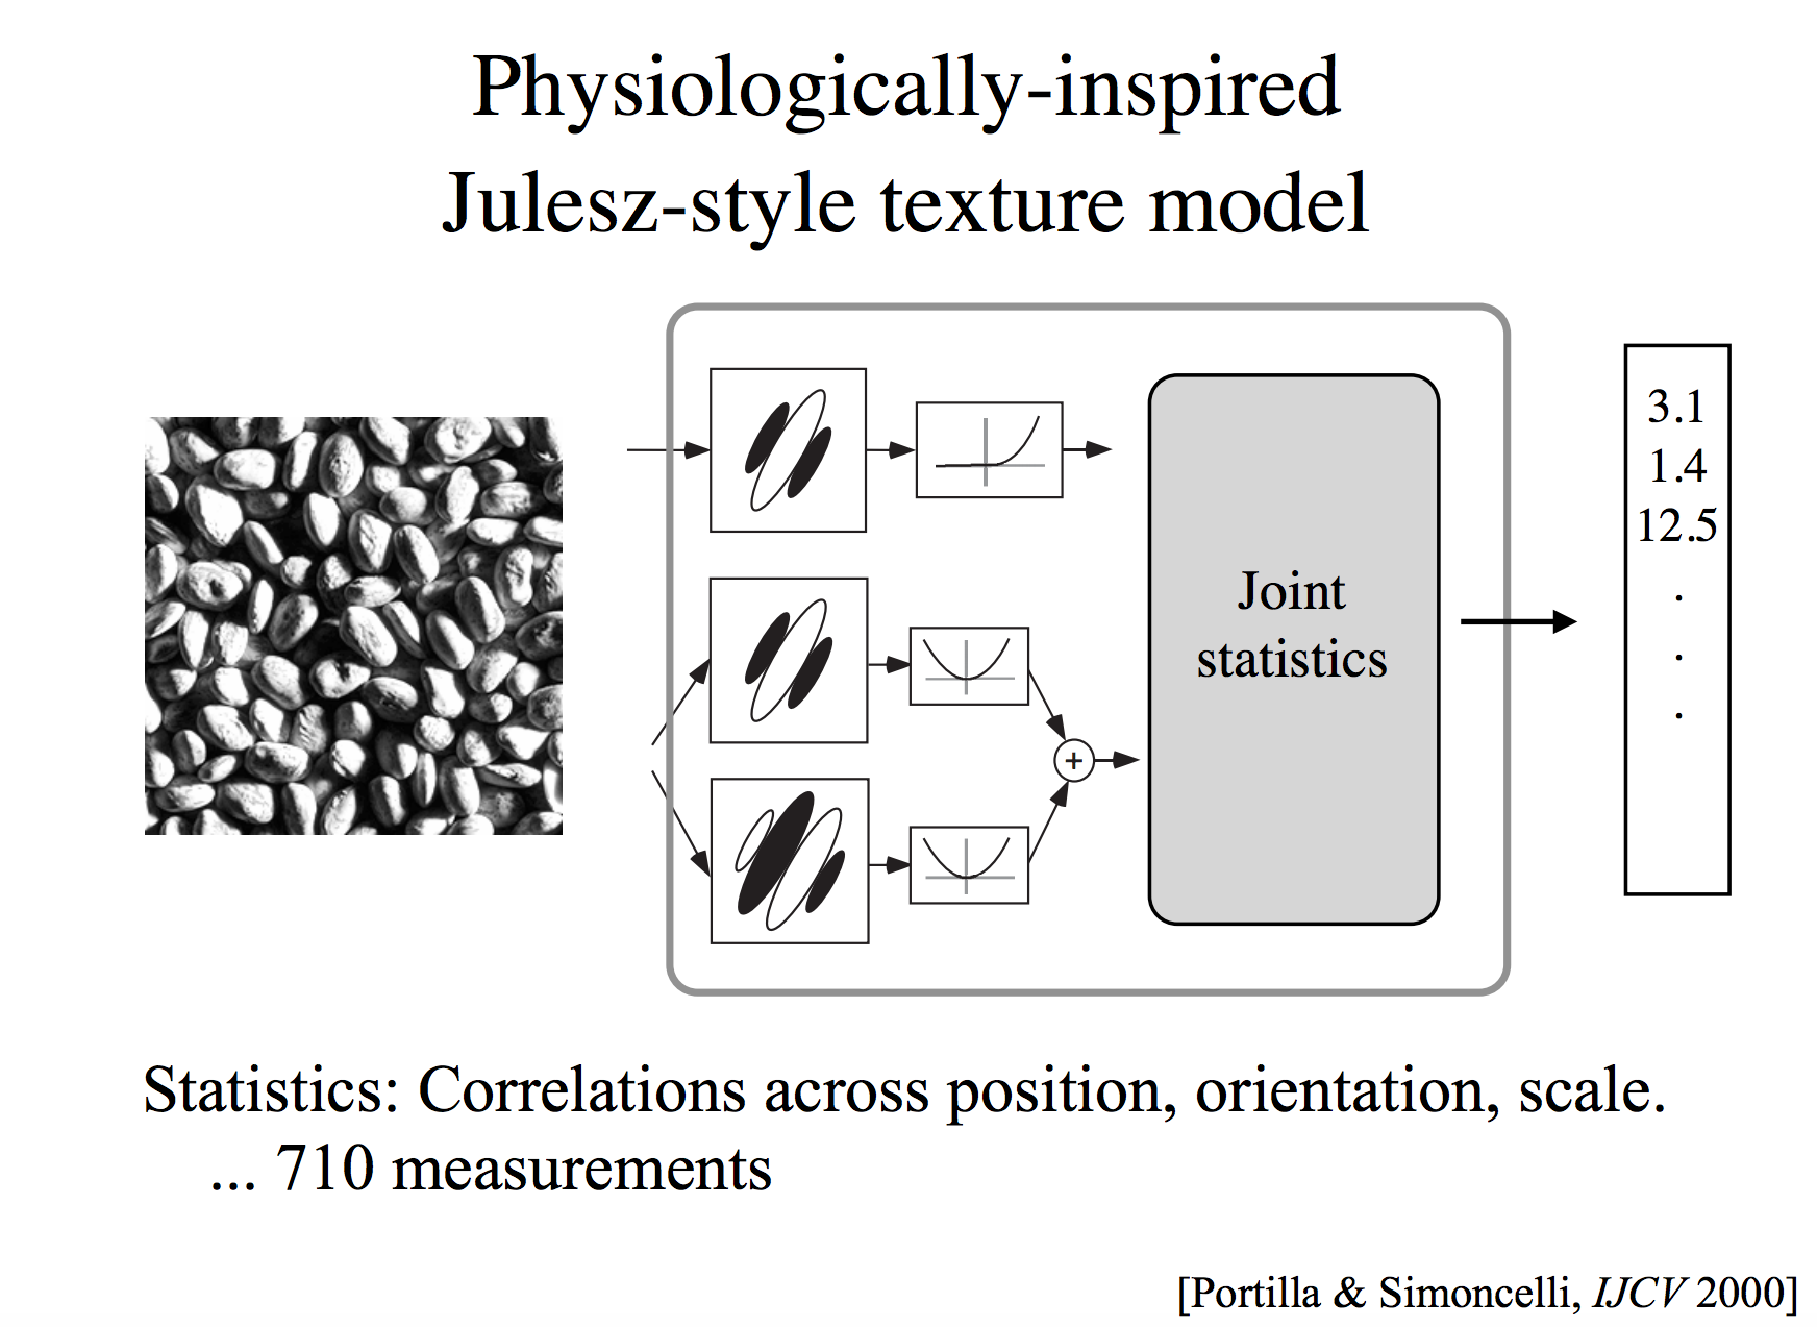
\includegraphics[width=0.9\textwidth]{figures/simoncelli-julesz-model} \\
\href{http://iclr.cc/lib/exe/fetch.php?media=iclr2017:simoncelli\_iclr2017.pdf}{\textcolor{blue}{Slides}}
\end{frame}

\begin{frame}{Invited Talk - Eero Simoncelli}
\centering
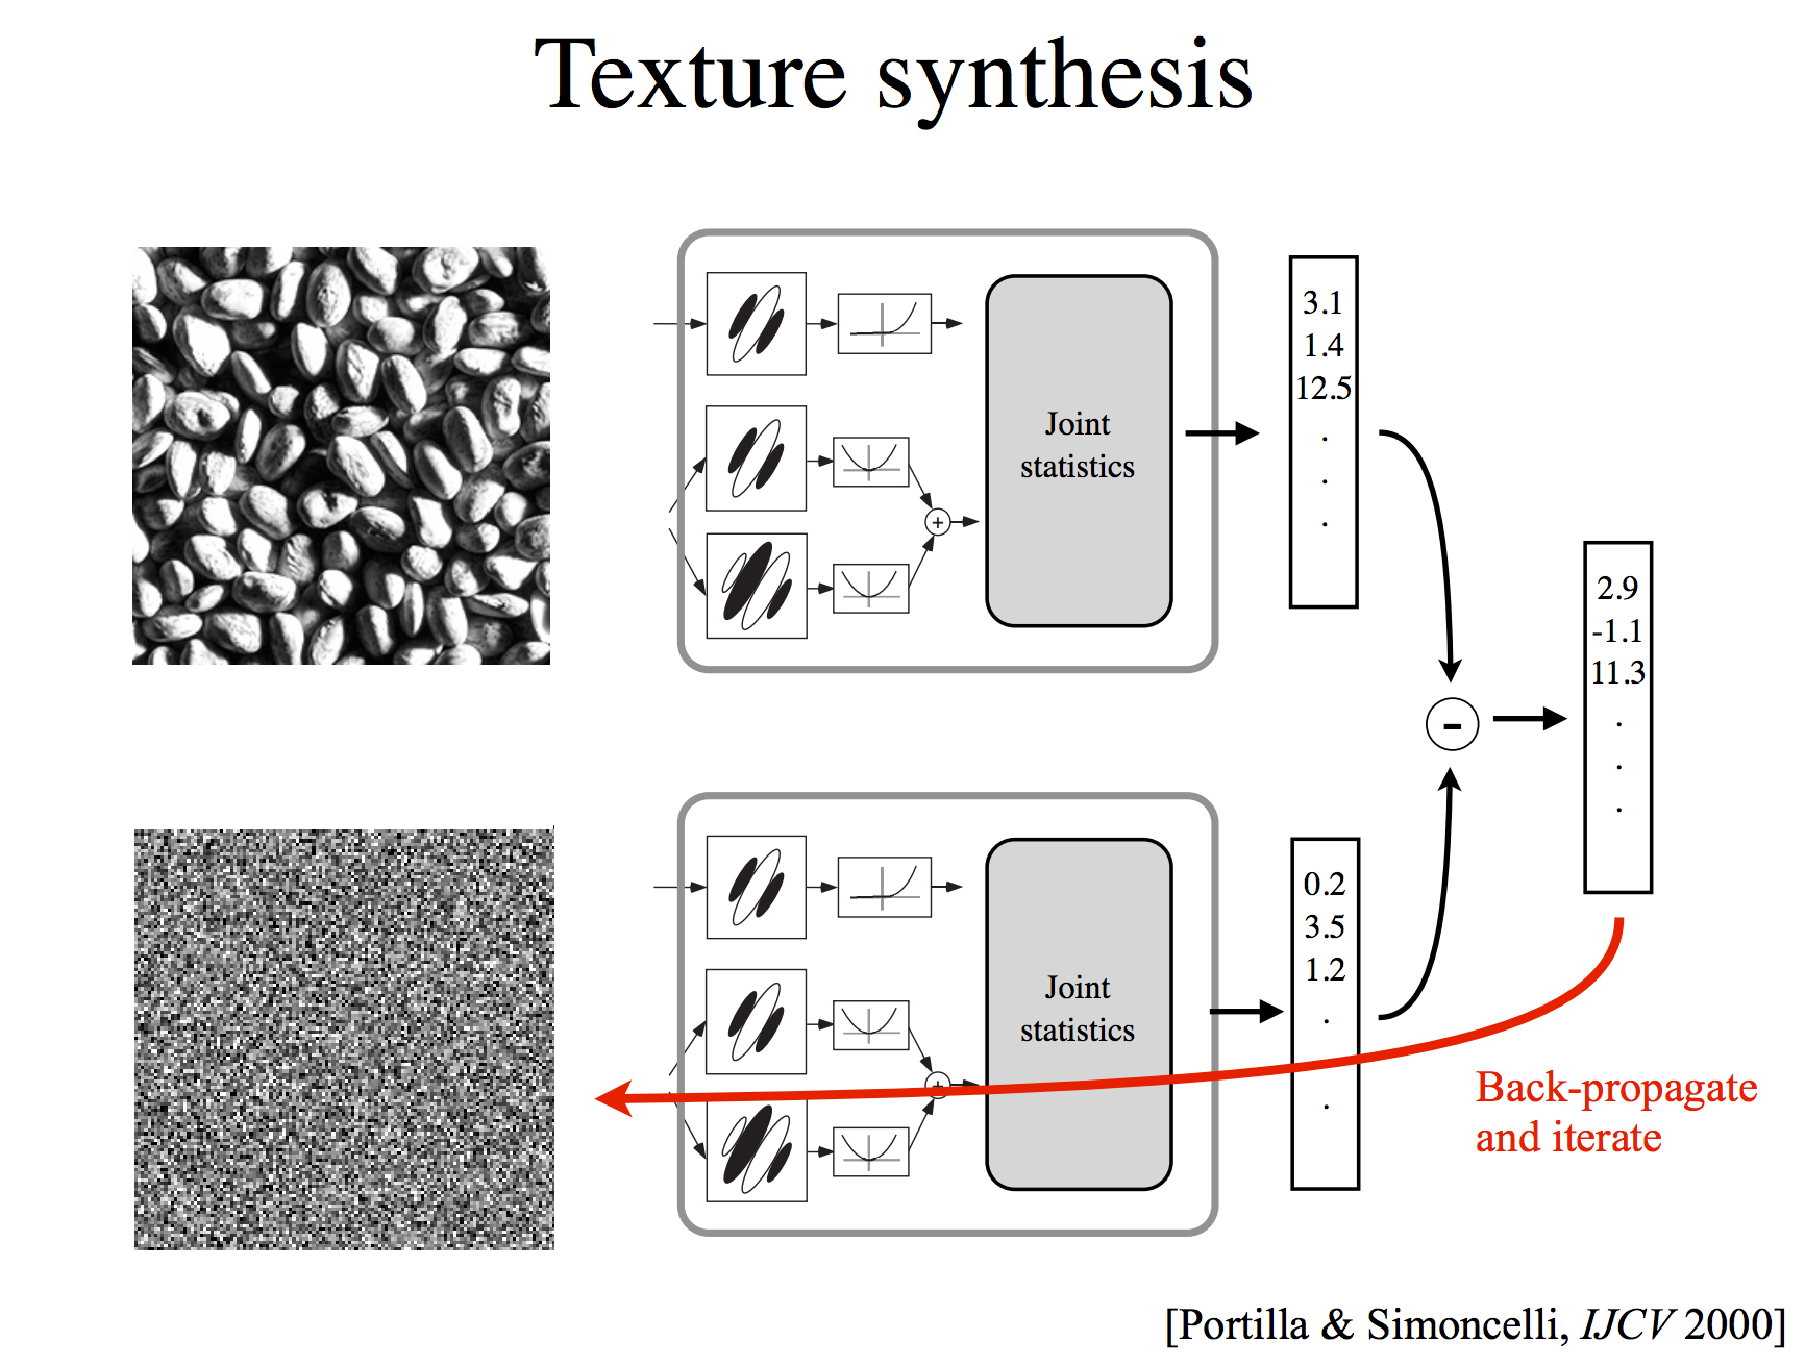
\includegraphics[width=0.9\textwidth]{figures/simoncelli-texture-synthesis} \\
\href{http://iclr.cc/lib/exe/fetch.php?media=iclr2017:simoncelli\_iclr2017.pdf}{\textcolor{blue}{Slides}}
\end{frame}

\begin{frame}{Invited Talk - Eero Simoncelli}
\centering
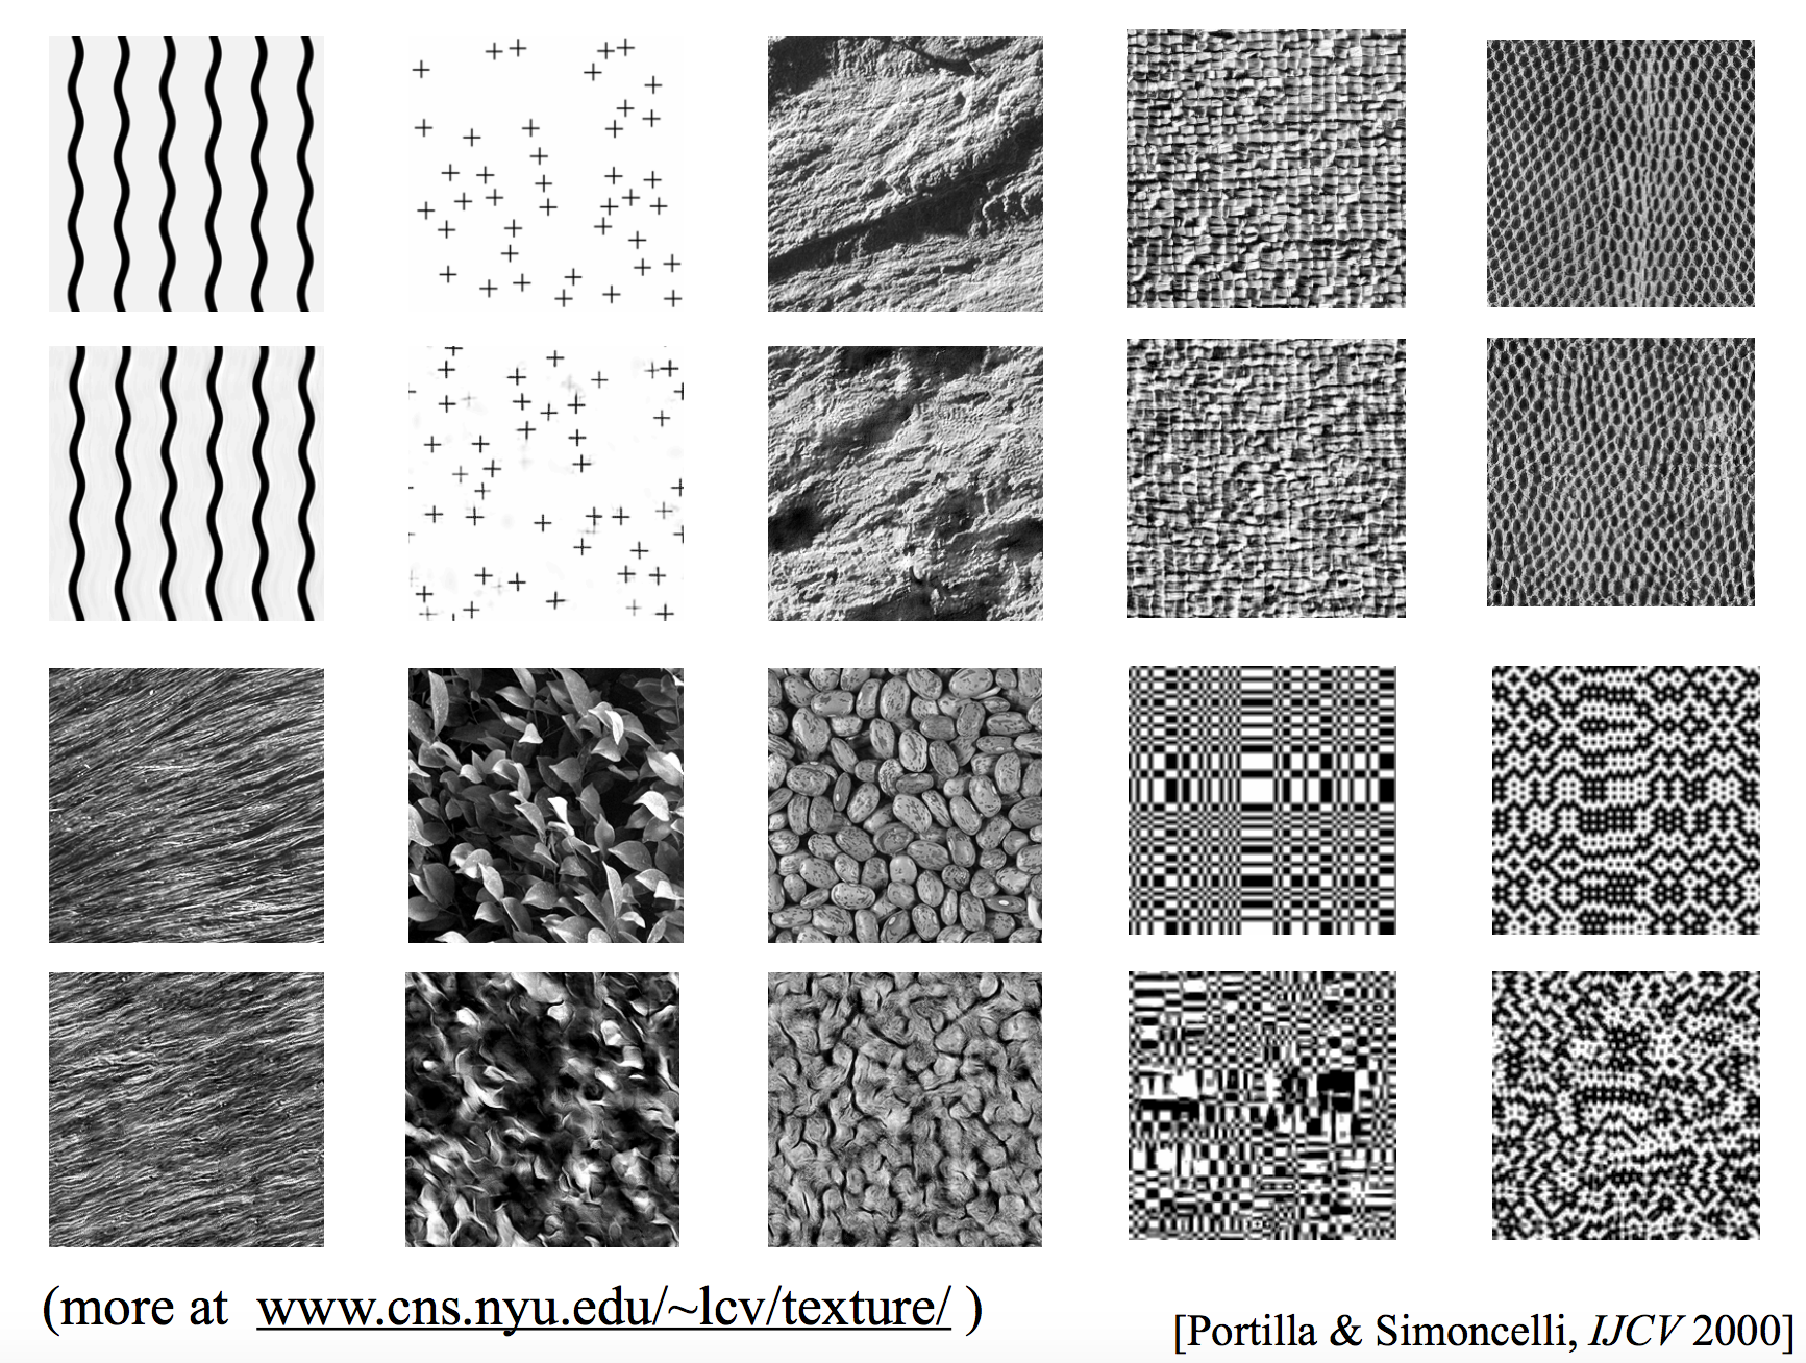
\includegraphics[width=0.9\textwidth]{figures/simoncelli-texture-synthesis-examples} \\
\href{http://iclr.cc/lib/exe/fetch.php?media=iclr2017:simoncelli\_iclr2017.pdf}{\textcolor{blue}{Slides}}
\end{frame}

\begin{frame}{End-to-end Optimized Image Compression}
\centering
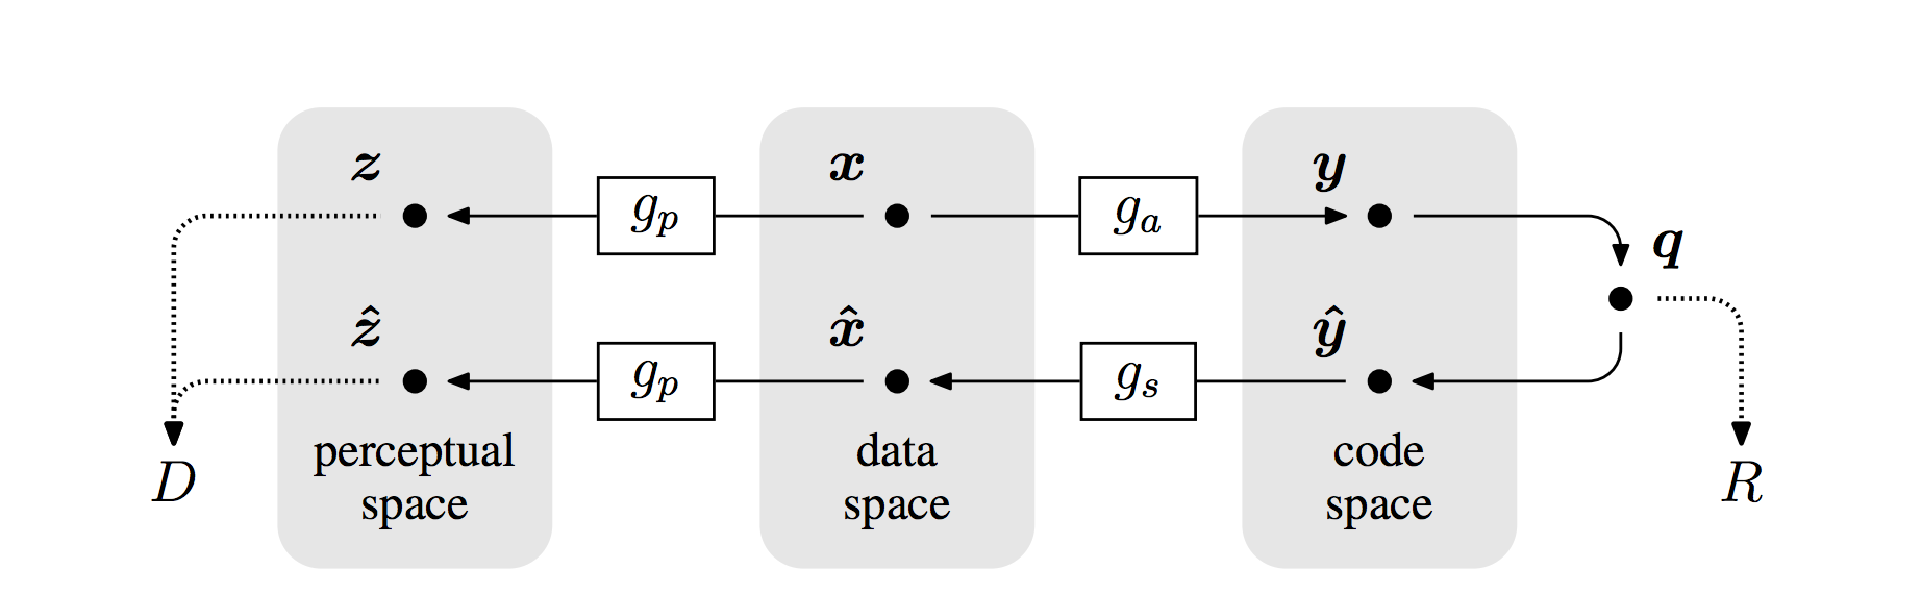
\includegraphics[width=0.9\textwidth]{figures/balle-framework} \\
\href{https://openreview.net/forum?id=rJxdQ3jeg}{\textcolor{blue}{Paper}}
\end{frame}

\begin{frame}{End-to-end Optimized Image Compression}
\centering
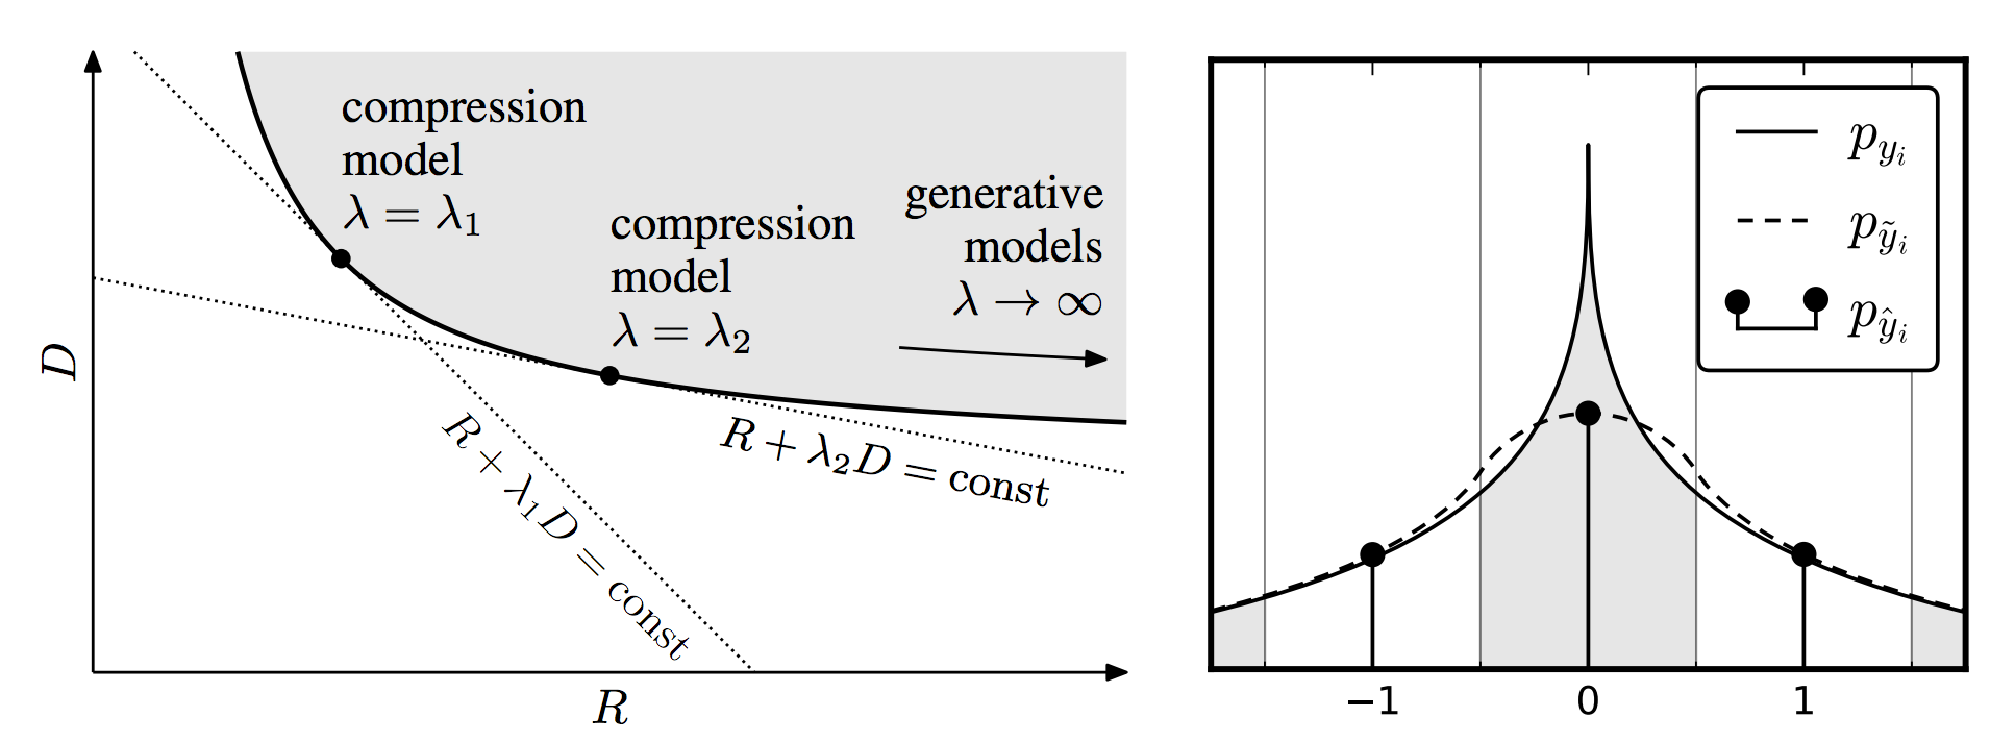
\includegraphics[width=0.9\textwidth]{figures/balle-tradeoff} \\
\href{https://openreview.net/forum?id=rJxdQ3jeg}{\textcolor{blue}{Paper}}
\end{frame}

\begin{frame}{Amortised MAP Inference for Image Super-resolution}
\centering
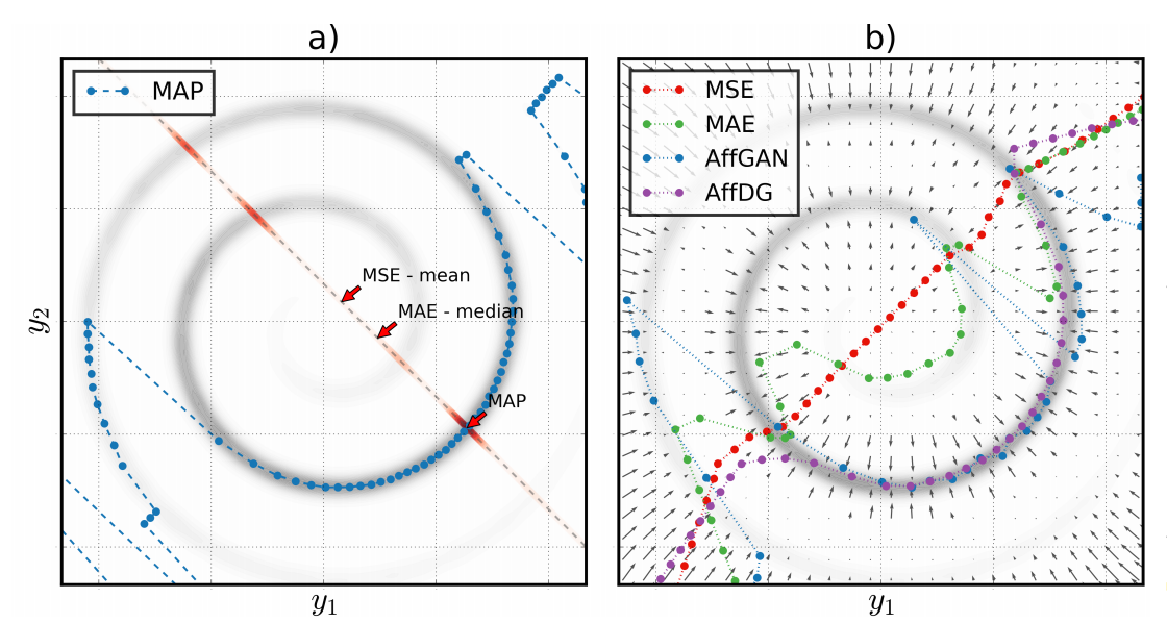
\includegraphics[width=0.9\textwidth]{figures/sonderby-swiss-roll} \\
\href{https://openreview.net/forum?id=S1RP6GLle}{\textcolor{blue}{Paper}}
\end{frame}

\begin{frame}{Amortised MAP Inference for Image Super-resolution}
\centering
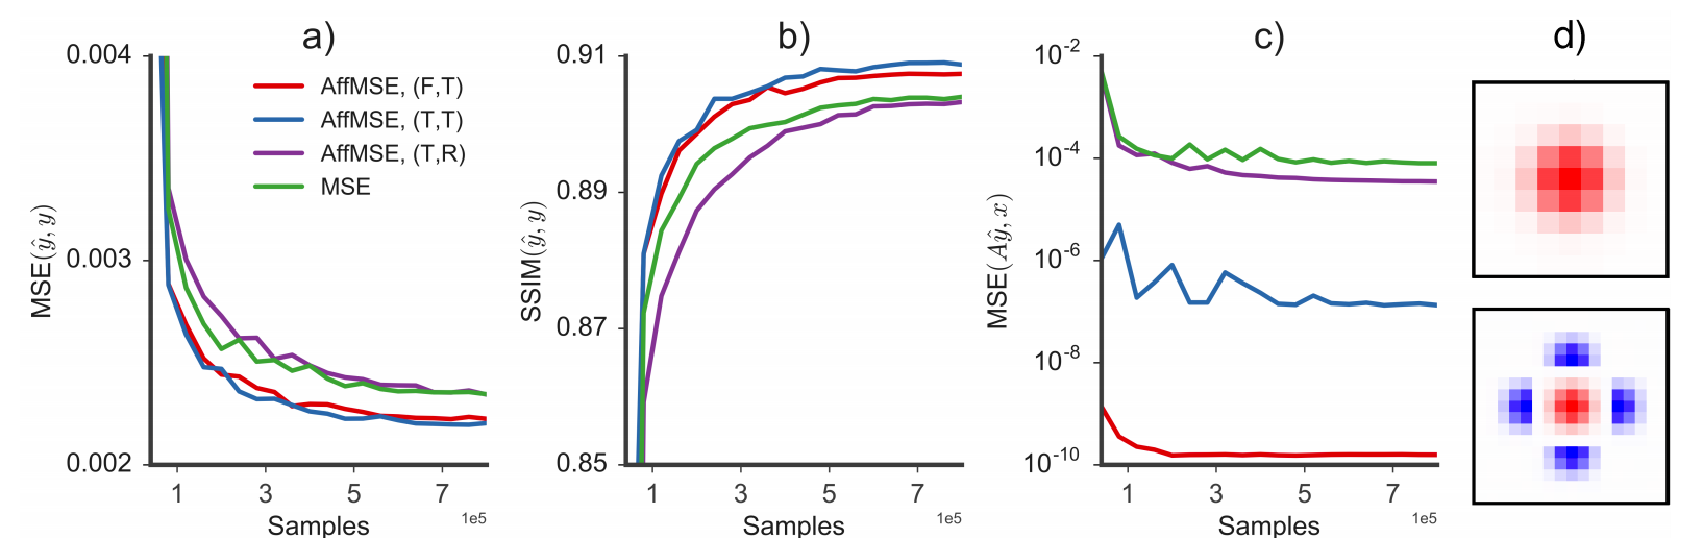
\includegraphics[width=0.9\textwidth]{figures/sonderby-celeba} \\
\href{https://openreview.net/forum?id=S1RP6GLle}{\textcolor{blue}{Paper}}
\end{frame}

\begin{frame}{Invited Talk - Benjamin Recht}
\centering
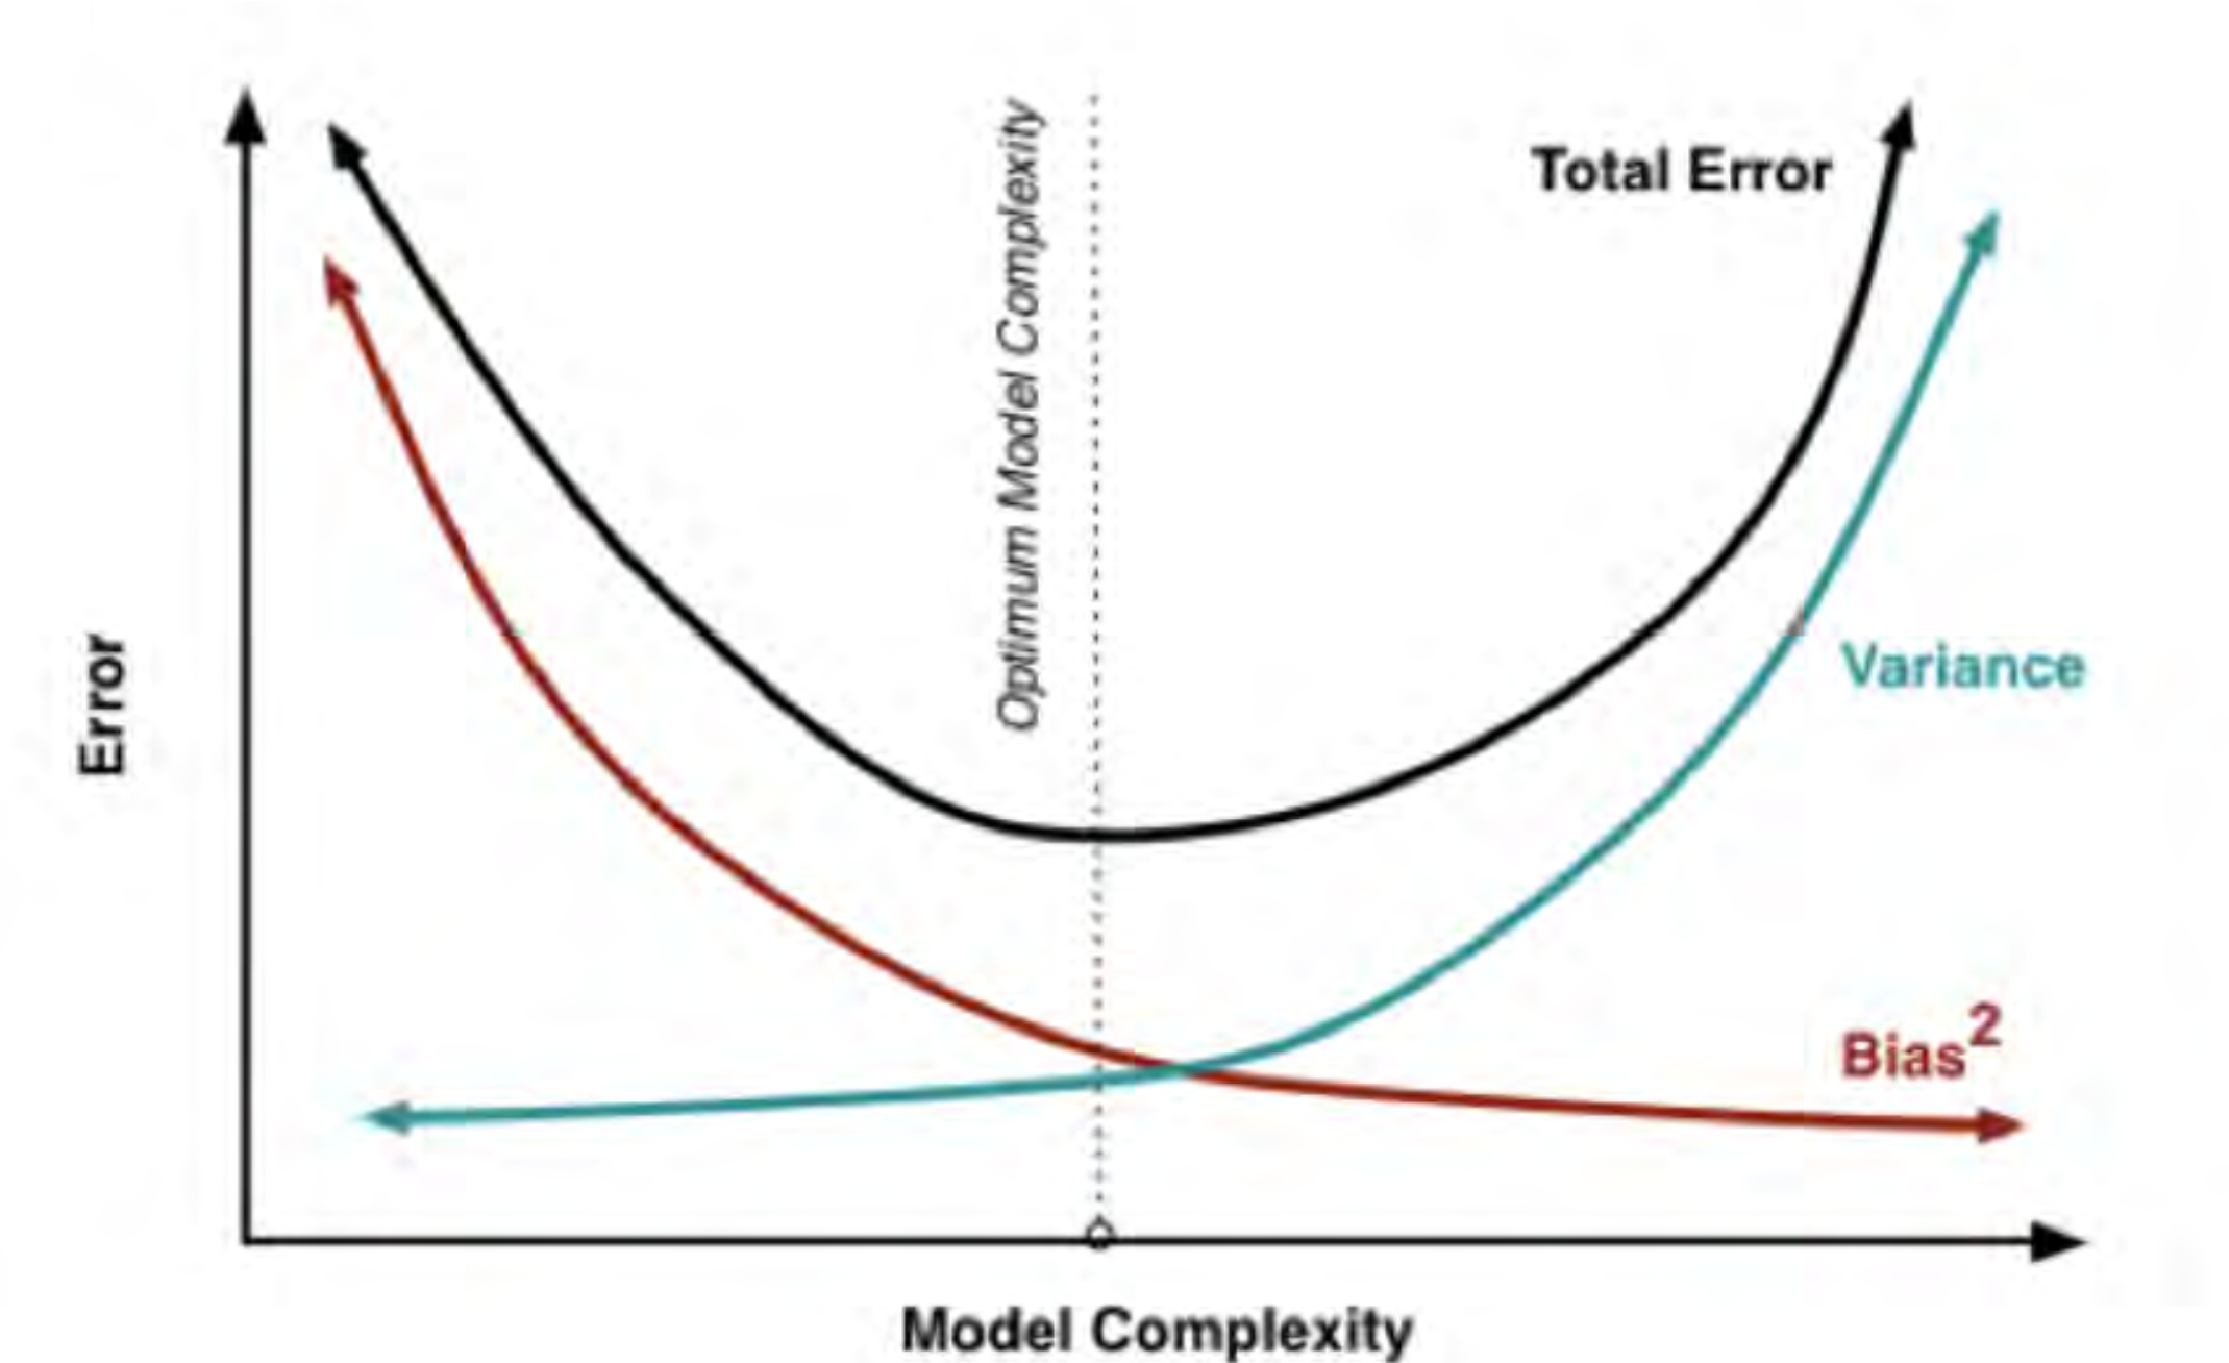
\includegraphics[width=0.9\textwidth]{figures/recht-bias-variance} \\
\href{http://iclr.cc/lib/exe/fetch.php?media=iclr2017:recht\_iclr2017.pdf}{\textcolor{blue}{Slides}}
\end{frame}

\begin{frame}{Invited Talk - Benjamin Recht}
\centering
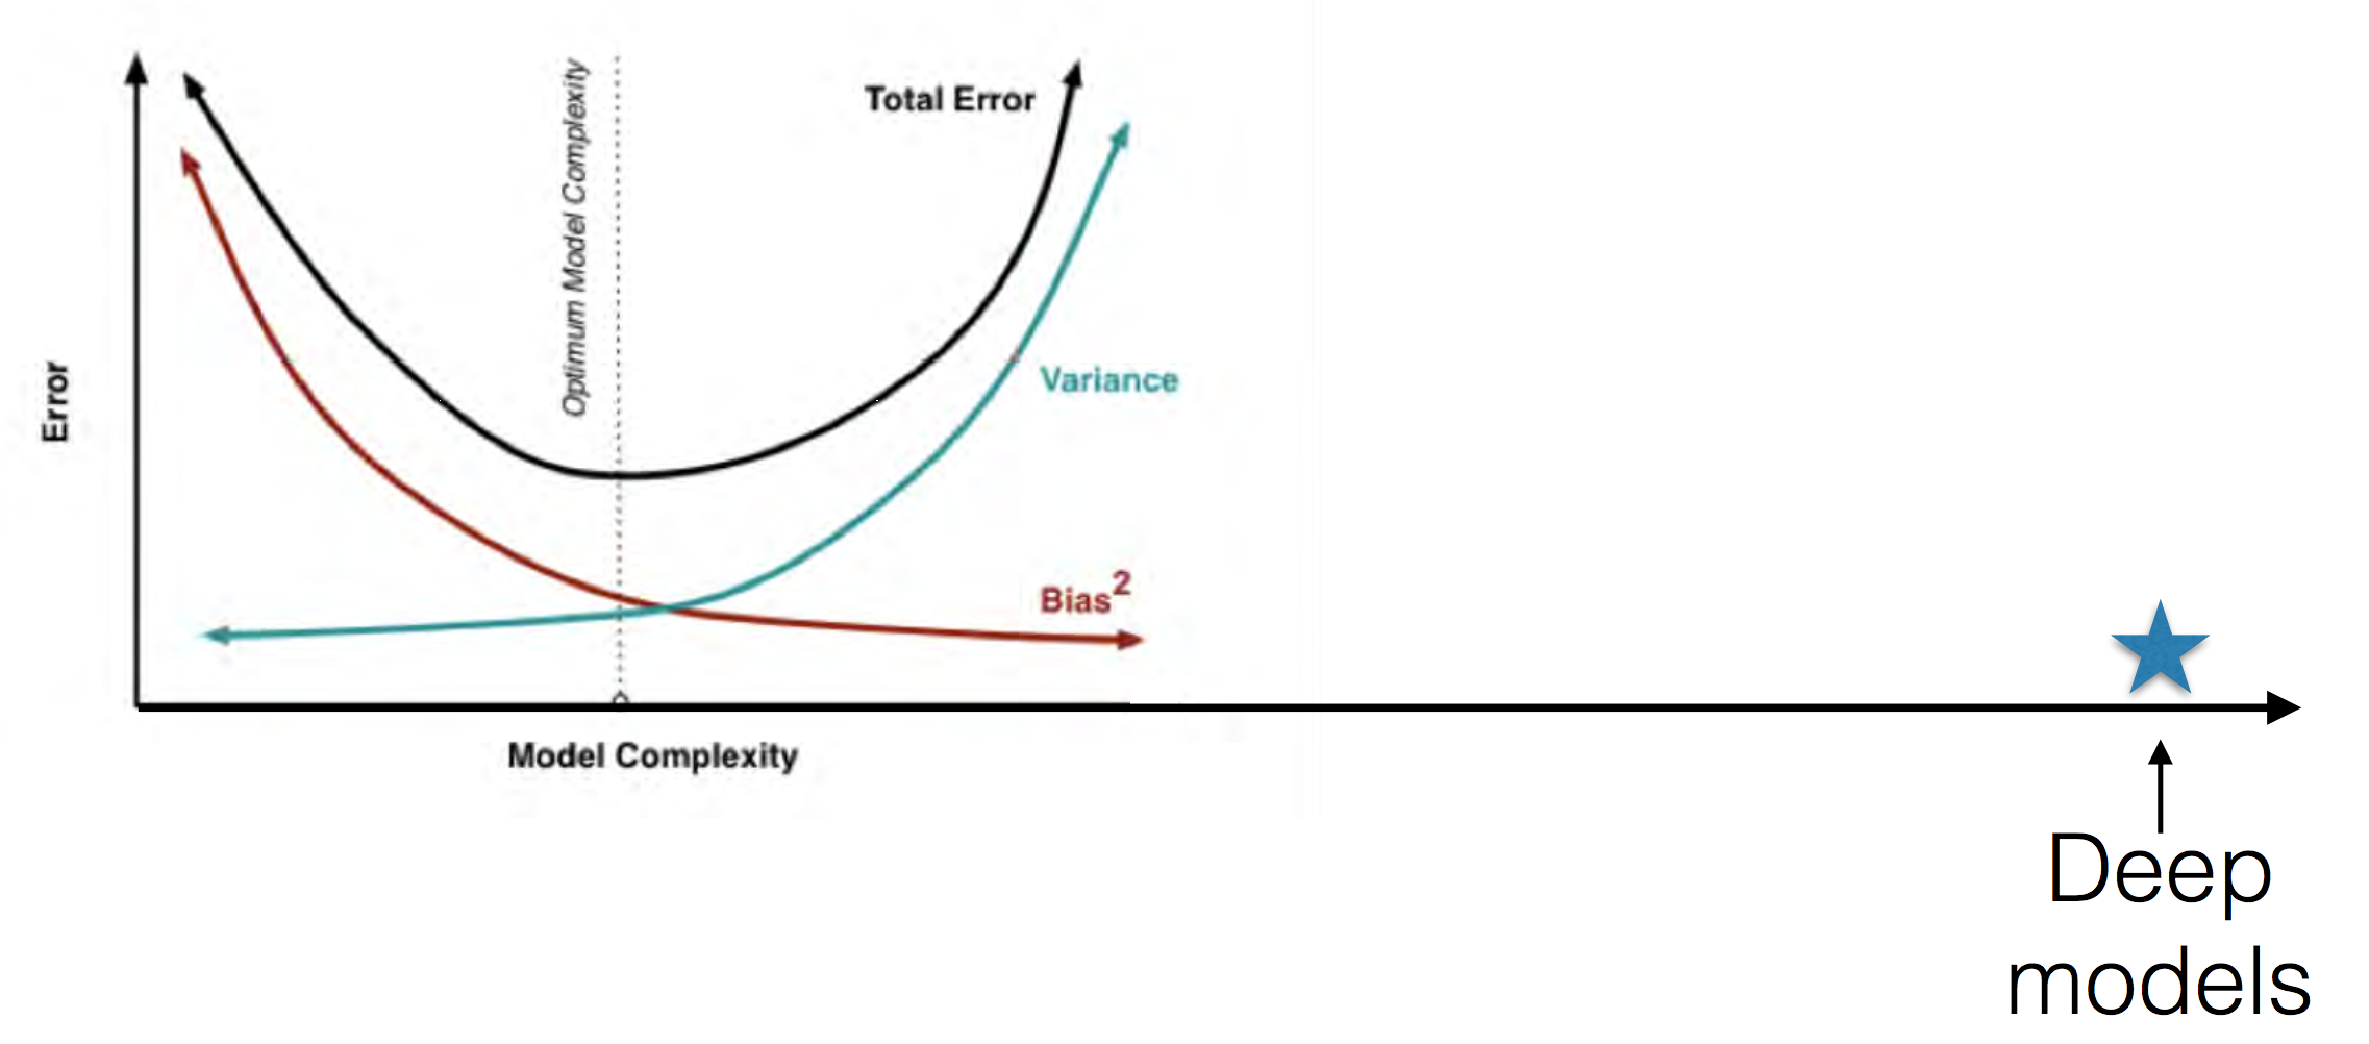
\includegraphics[width=0.9\textwidth]{figures/recht-bias-variance-conundrum} \\
\href{http://iclr.cc/lib/exe/fetch.php?media=iclr2017:recht\_iclr2017.pdf}{\textcolor{blue}{Slides}}
\end{frame}

\begin{frame}{Understanding Deep Learning Requires Rethinking Generalization}
\centering
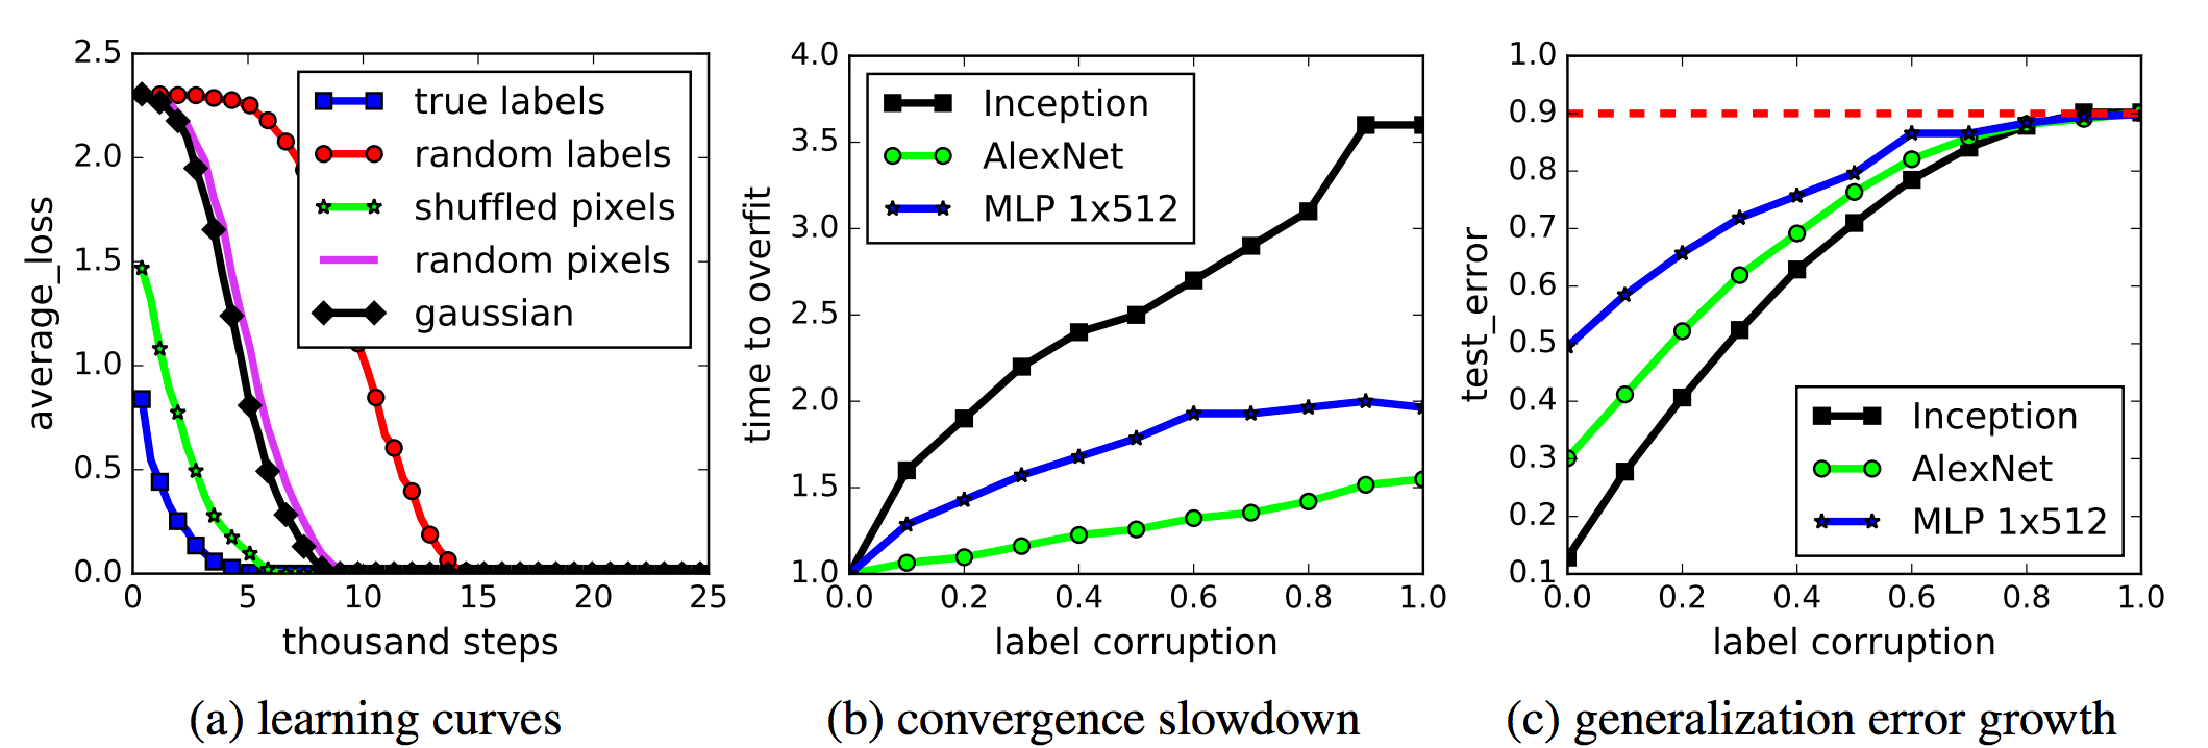
\includegraphics[width=0.9\textwidth]{figures/zhang-learning-curves} \\
\href{http://openreview.net/forum?id=Sy8gdB9xx}{\textcolor{blue}{Paper}}
\end{frame}

\begin{frame}{Background: Flat Minima}
\centering
\includegraphics[width=0.9\textwidth]{figures/hochreiter-flat-sharp} \\
\href{http://www.bioinf.jku.at/publications/older/3304.pdf}{\textcolor{blue}{Paper}}
\end{frame}

\begin{frame}{Large-Batch Training for Deep Learning: Generalization Gap and Sharp Minima}

\centering
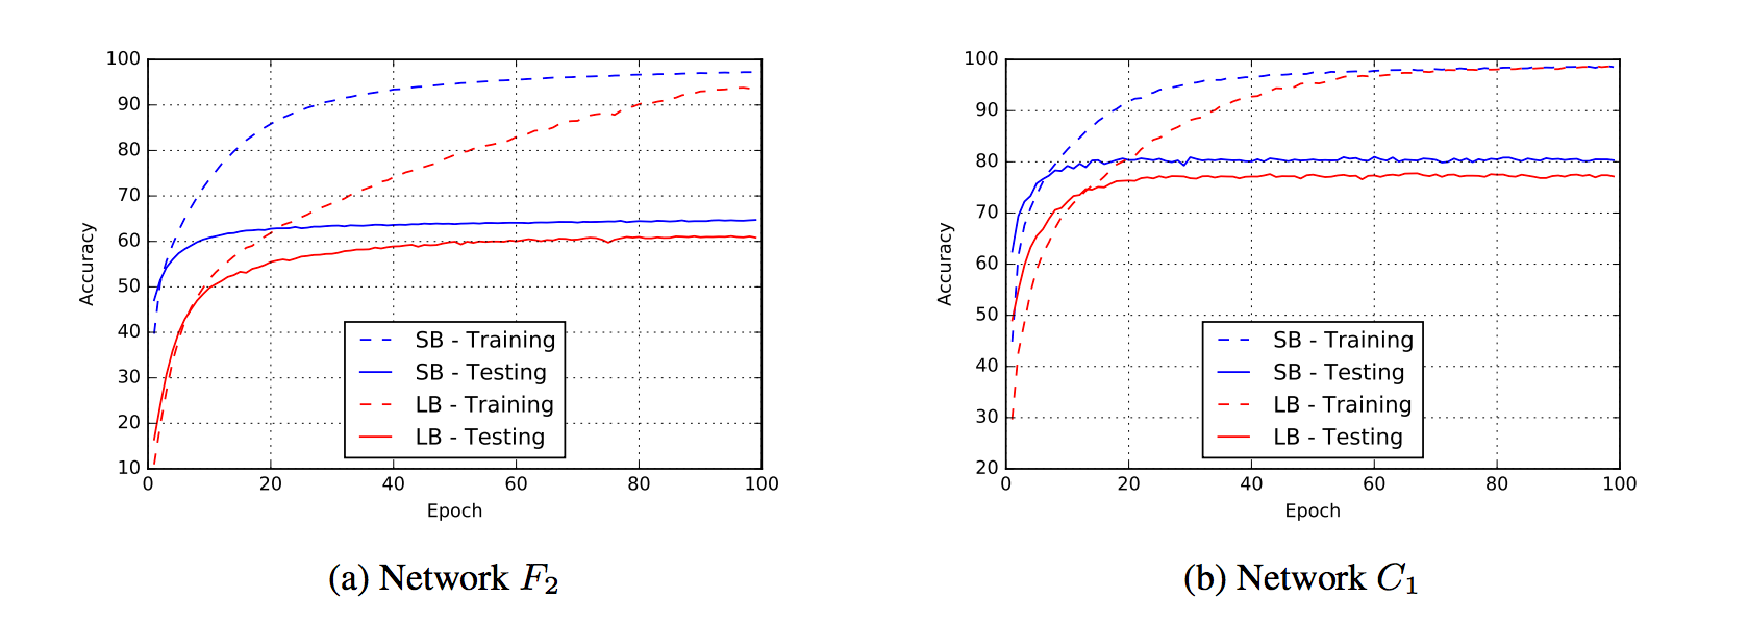
\includegraphics[width=0.9\textwidth]{figures/keskar-learning-curves-concept} \\
\href{https://openreview.net/forum?id=H1oyRlYgg}{\textcolor{blue}{Paper}}
\end{frame}

\begin{frame}{Large-Batch Training for Deep Learning: Generalization Gap and Sharp Minima}
\centering
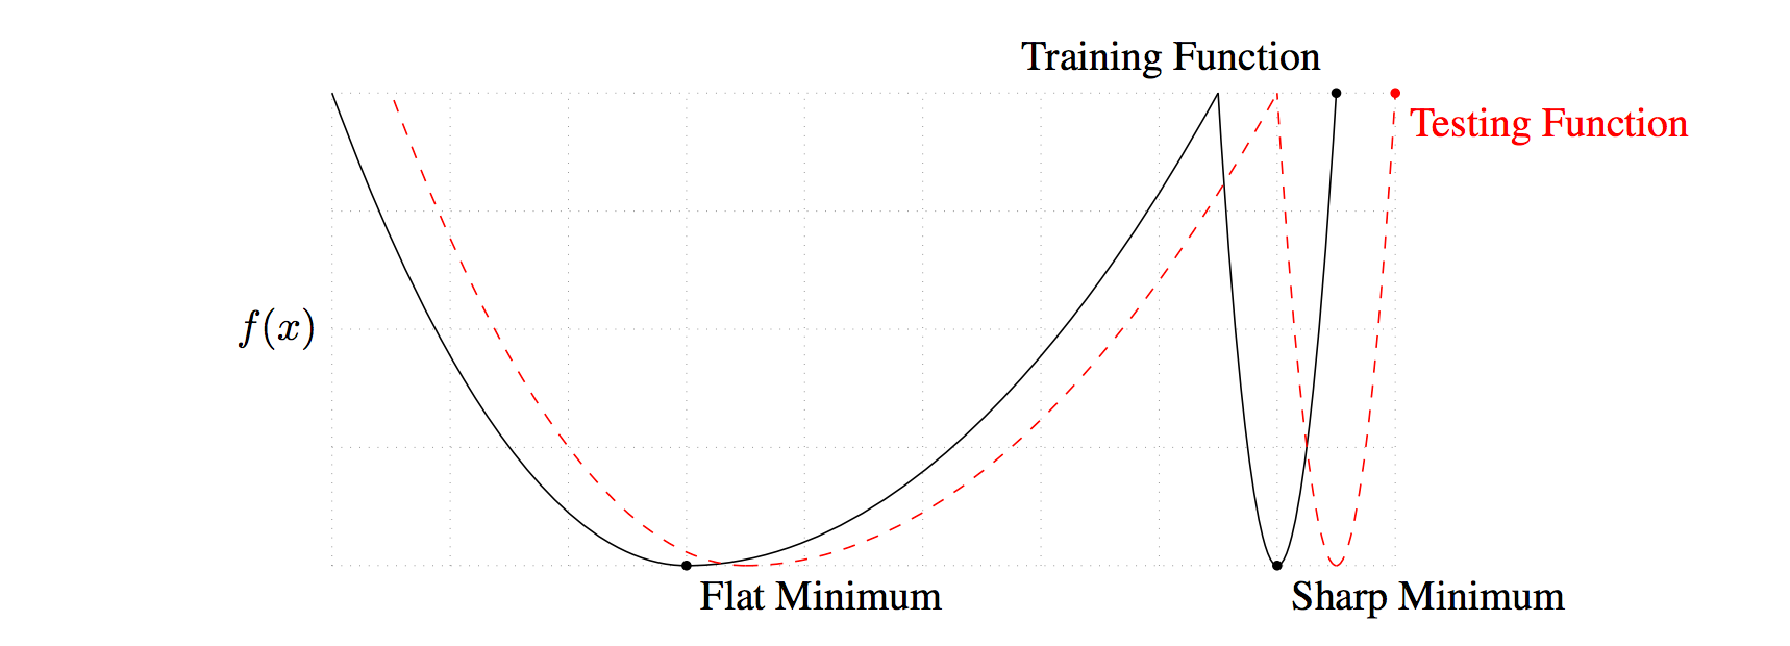
\includegraphics[width=0.9\textwidth]{figures/keskar-flat-minima-concept} \\
\href{https://openreview.net/forum?id=H1oyRlYgg}{\textcolor{blue}{Paper}}
\end{frame}

\begin{frame}{Large-Batch Training for Deep Learning: Generalization Gap and Sharp Minima}
\centering
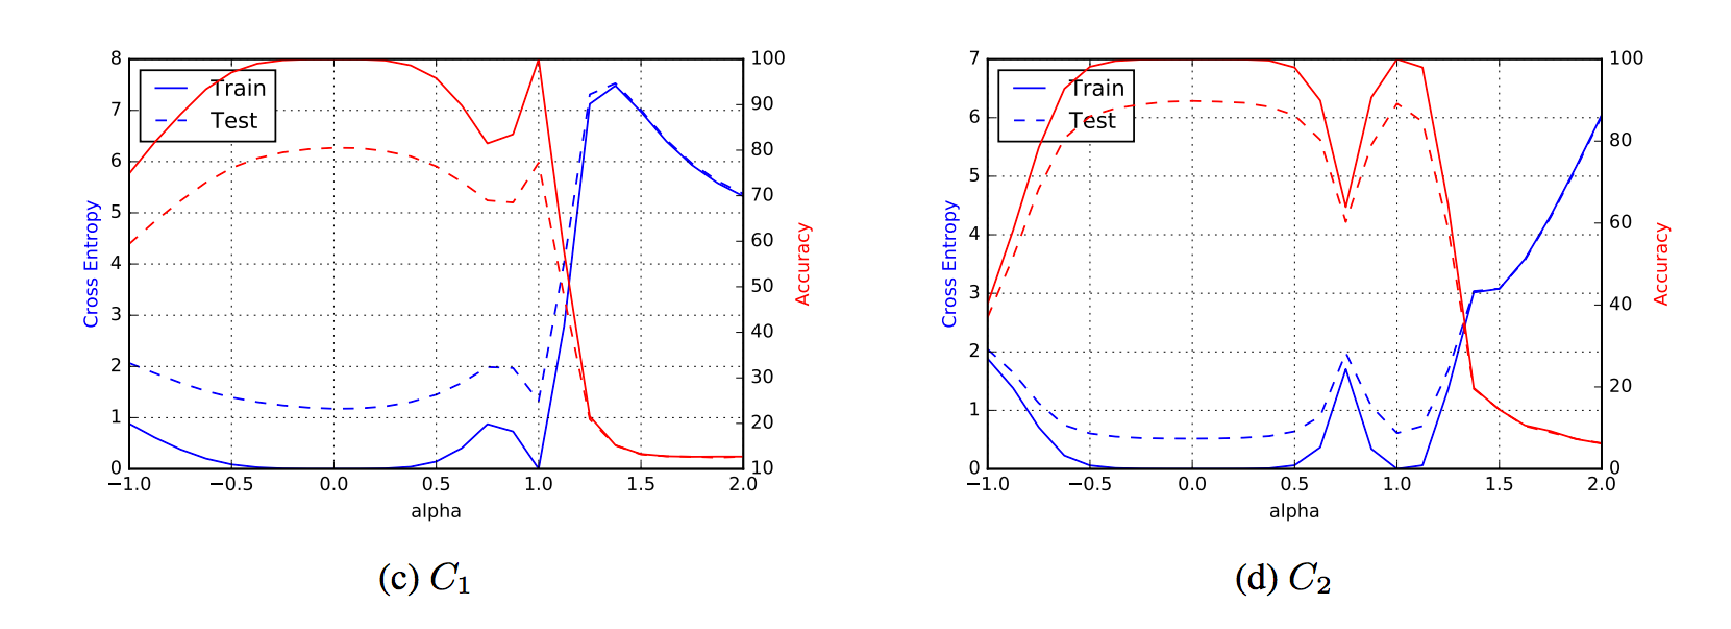
\includegraphics[width=0.9\textwidth]{figures/keskar-parametric-plots} \\
\href{https://openreview.net/forum?id=H1oyRlYgg}{\textcolor{blue}{Paper}}
\end{frame}

%\begin{frame}{Invited Talk - Riccardo Zecchina}
%\centering
%\href{http://iclr.cc/lib/exe/fetch.php?media=iclr2017:zecchina\_iclr2017.pdf}{\textcolor{blue}{Slides}}
%\end{frame}

%\begin{frame}{Contributed Talk}
%\centering
%%\includegraphics[width=0.9\textwidth]{figures/TODO} \\
%\href{https://openreview.net/forum?id=rJLS7qKel}
%{\textcolor{blue}{Learning to Act by Predicting the Future}}
%\end{frame}
%
%\begin{frame}{Contributed Talk}
%\centering
%%\includegraphics[width=0.9\textwidth]{figures/TODO} \\
%\href{https://openreview.net/forum?id=SJ6yPD5xg}{\textcolor{blue}{Learning with Unsupervised Auxiliary Tasks}}Pap
%\end{frame}
%
%\begin{frame}{Contributed Talk}
%\centering
%%\includegraphics[width=0.9\textwidth]{figures/TODO} \\
%\href{https://openreview.net/forum?id=SJ3rcZcxl}{\textcolor{blue}{Q-Prop: Sample-Efficient Policy Gradient with An Off-Policy Critic}}
%\end{frame}
%
%\begin{frame}{Contributed Talk}
%\centering
%%\includegraphics[width=0.9\textwidth]{figures/TODO} \\
%\href{https://openreview.net/forum?id=S1Bb3D5gg}{\textcolor{blue}{Learning End-to-End Goal-Oriented Dialog}}
%\end{frame}
%
%\begin{frame}{Contributed Talk}
%\centering
%%\includegraphics[width=0.9\textwidth]{figures/TODO} \\
%\href{https://openreview.net/forum?id=Hk8N3Sclg}{\textcolor{blue}{Multi-Agent Cooperation and the Emergence of (Natural) Language}}
%\end{frame}

\begin{frame}{Invited Talk - Alex Graves}
\centering
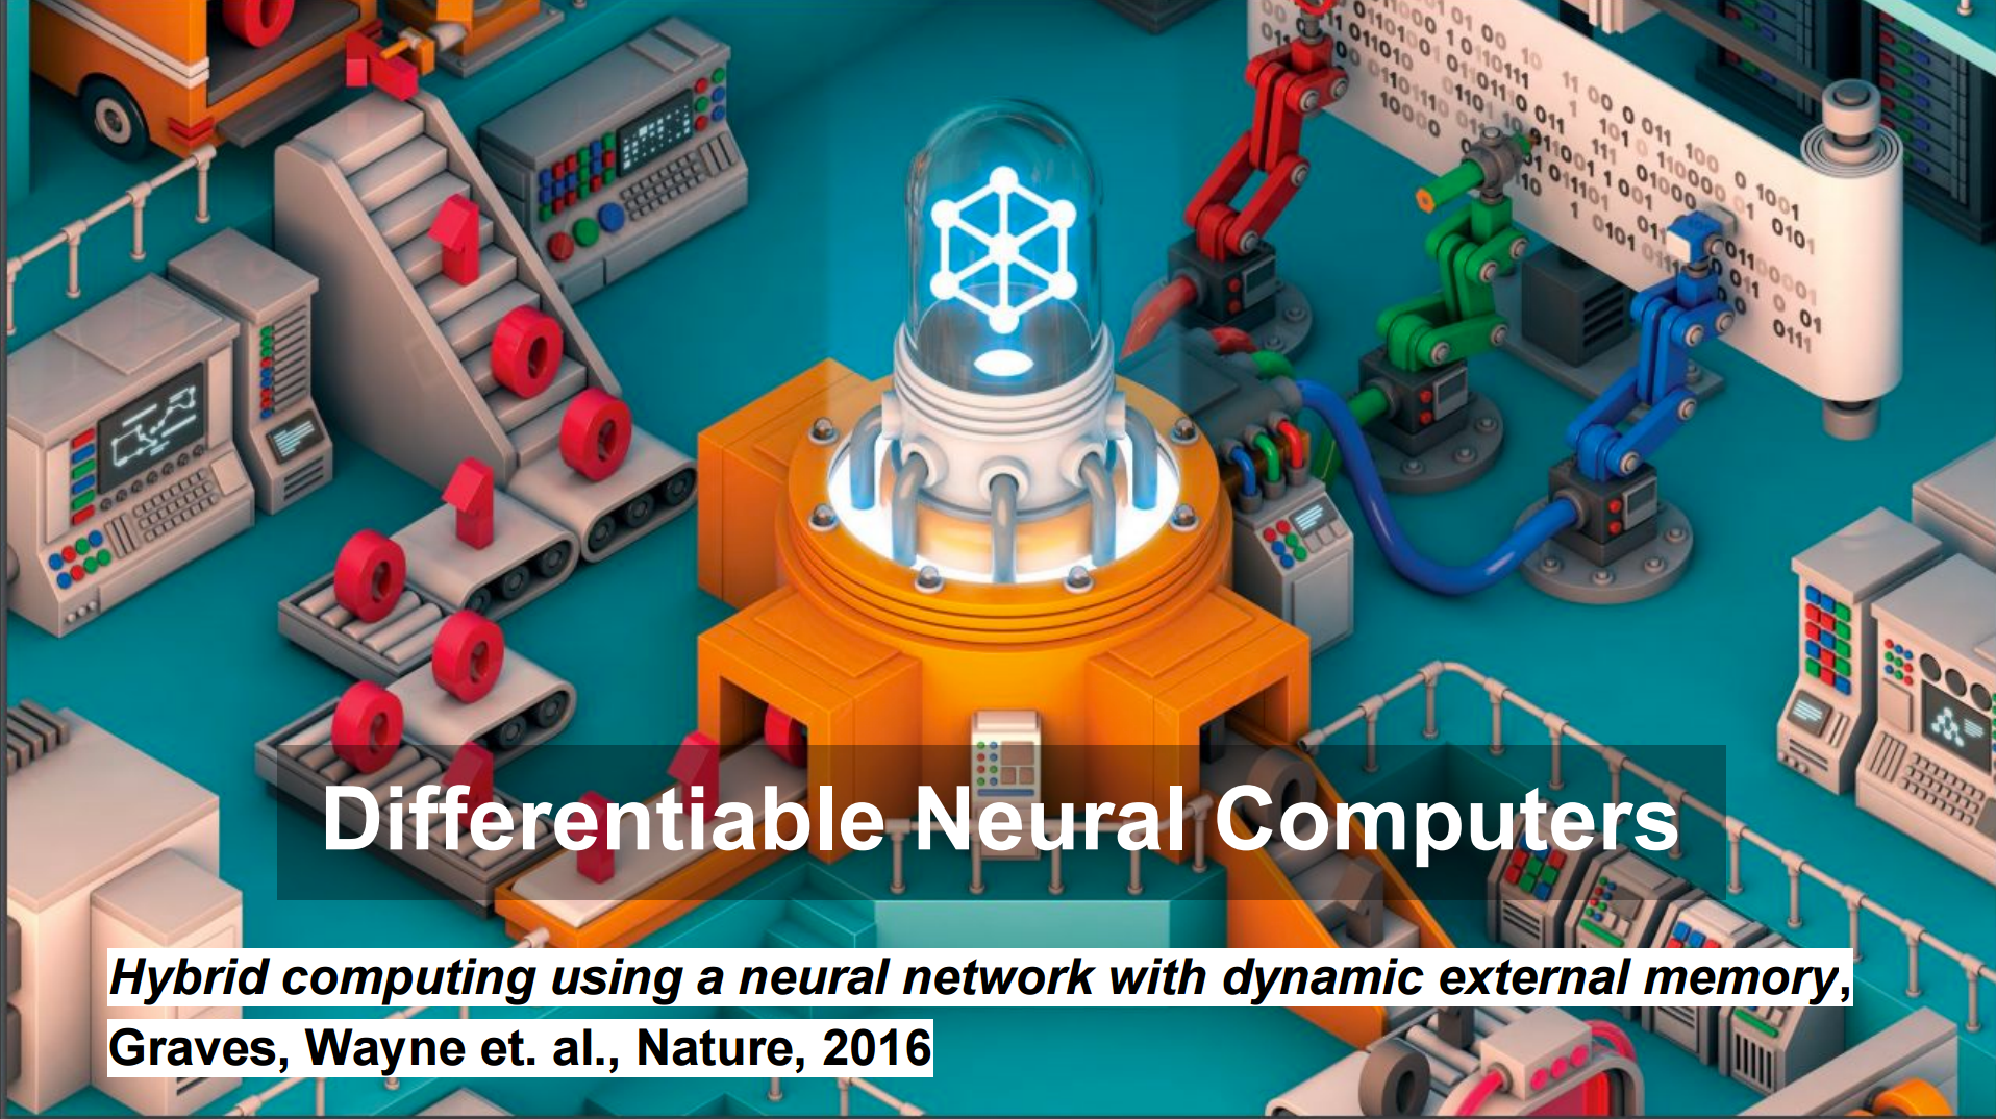
\includegraphics[width=0.9\textwidth]{figures/graves-nature} \\
\href{http://iclr.cc/lib/exe/fetch.php?media=iclr2017:graves\_iclr2017.pdf}{\textcolor{blue}{Slides}}
\end{frame}

\begin{frame}{Invited Talk - Alex Graves}
\centering
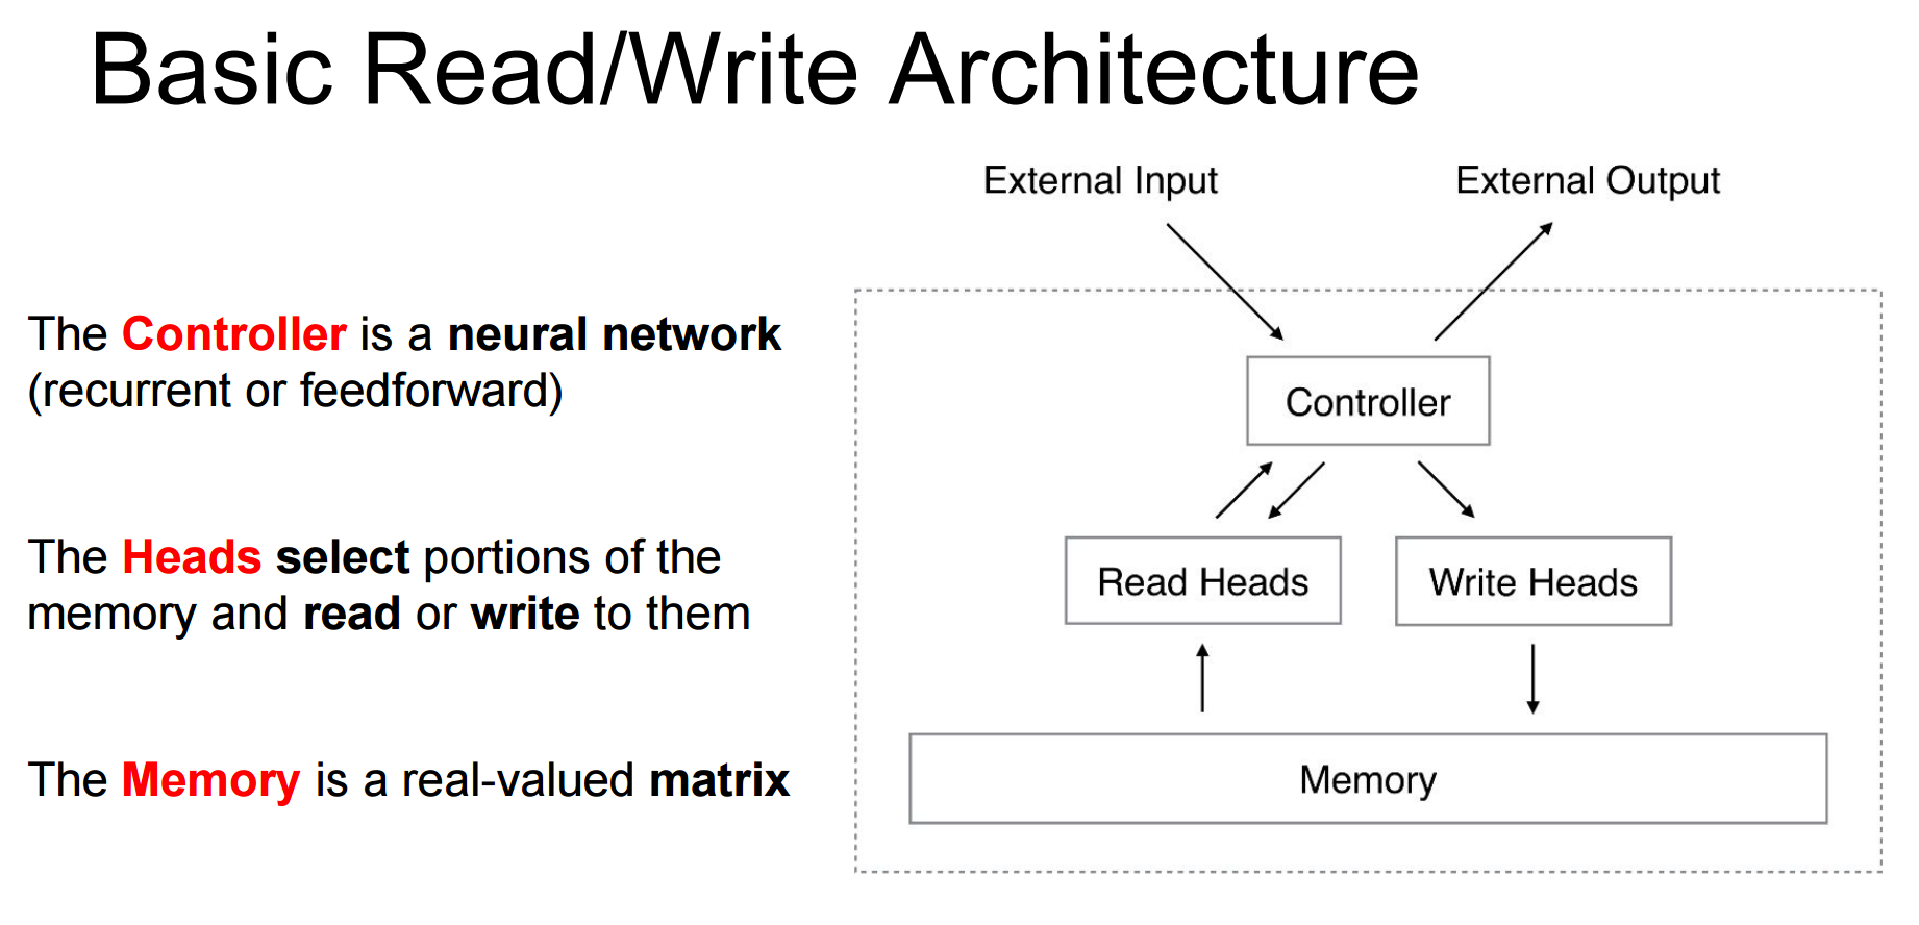
\includegraphics[width=0.9\textwidth]{figures/graves-architecture} \\
\href{http://iclr.cc/lib/exe/fetch.php?media=iclr2017:graves\_iclr2017.pdf}{\textcolor{blue}{Slides}}
\end{frame}

\begin{frame}{Invited Talk - Alex Graves}
\centering
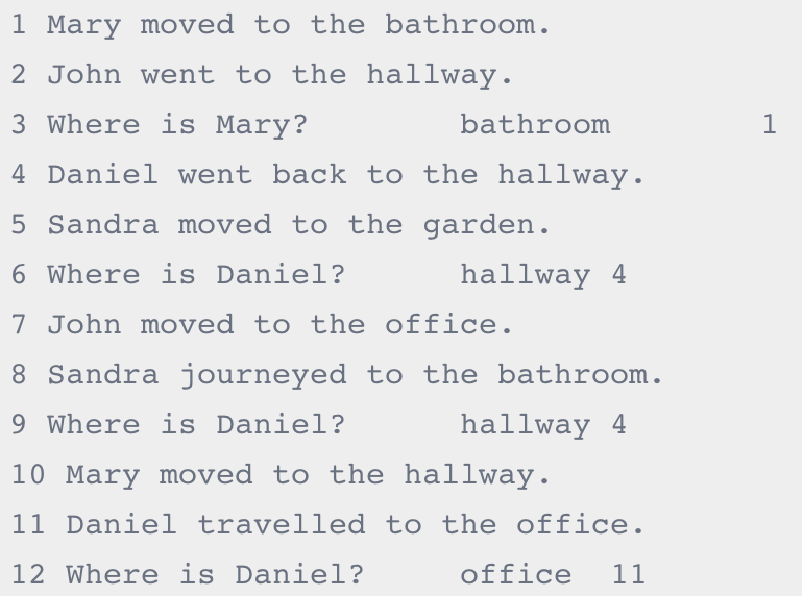
\includegraphics[width=0.9\textwidth]{figures/graves-babi} \\
\href{http://iclr.cc/lib/exe/fetch.php?media=iclr2017:graves\_iclr2017.pdf}{\textcolor{blue}{Slides}}
\end{frame}

\begin{frame}{Invited Talk - Alex Graves}
\centering
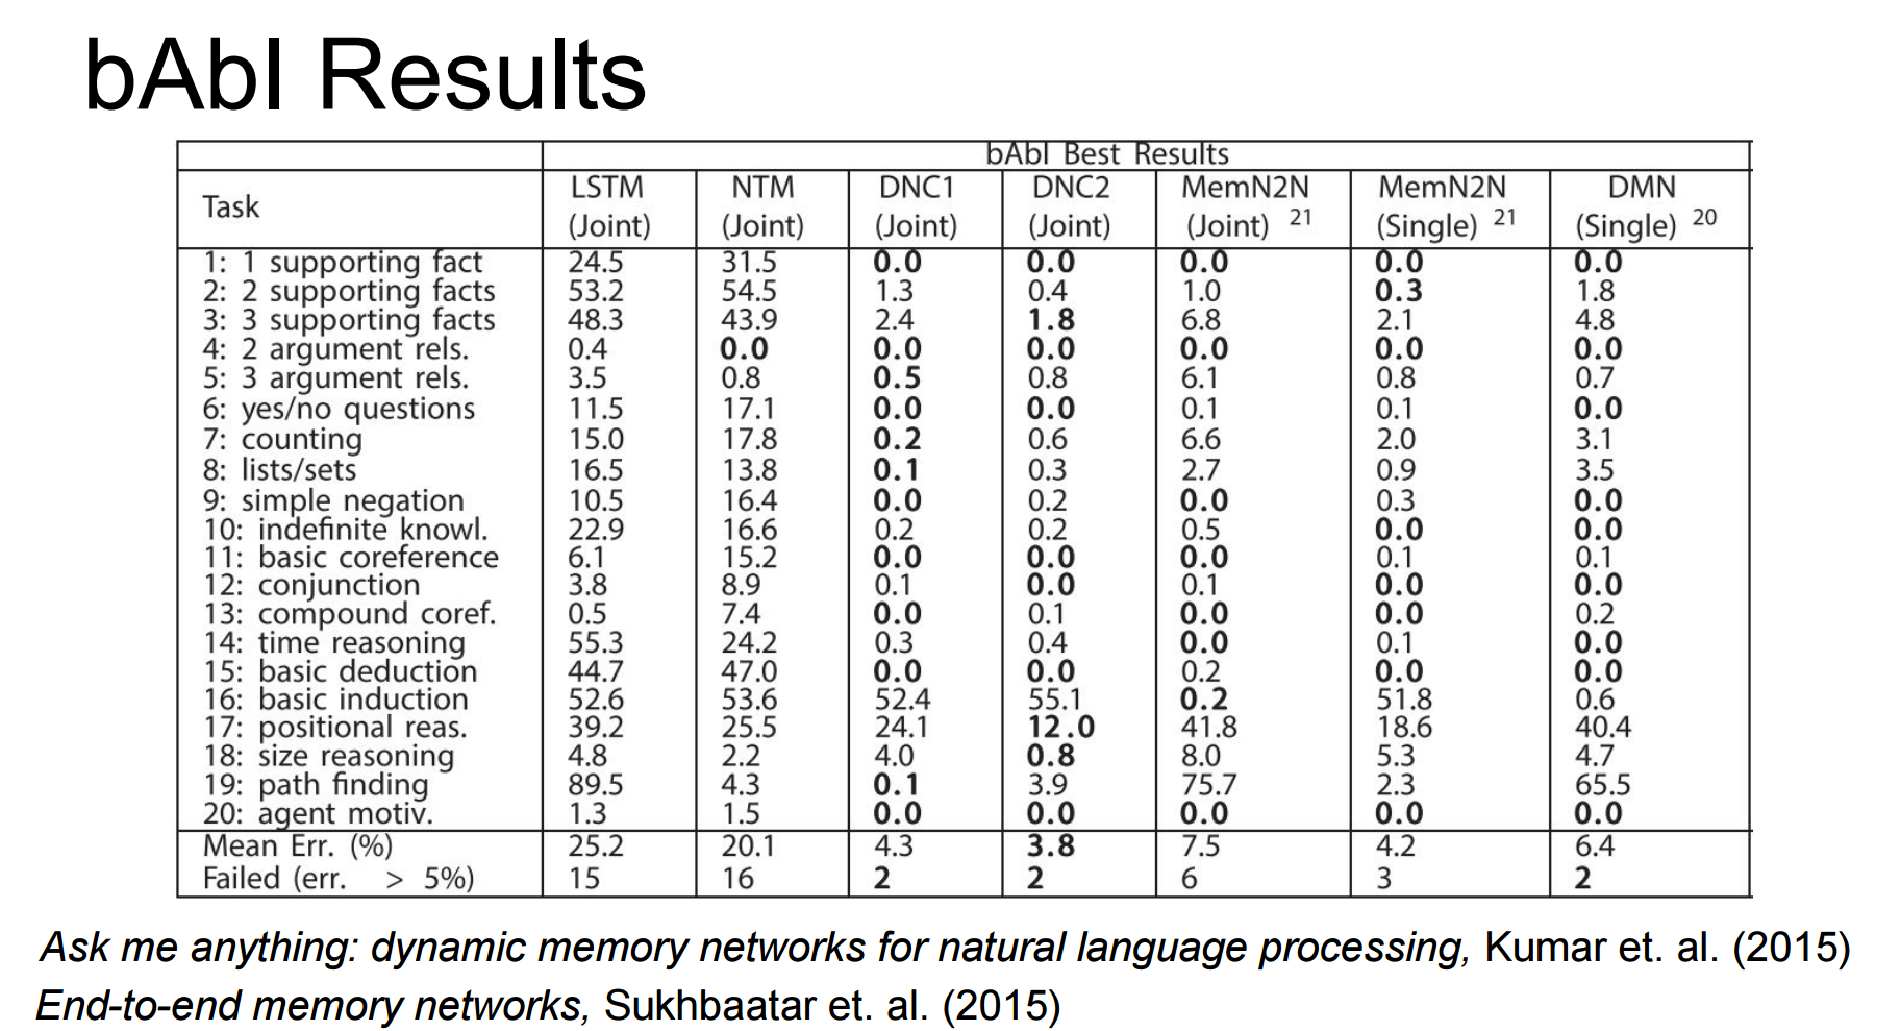
\includegraphics[width=0.9\textwidth]{figures/graves-results} \\
\href{http://iclr.cc/lib/exe/fetch.php?media=iclr2017:graves\_iclr2017.pdf}{\textcolor{blue}{Slides}}
\end{frame}

\begin{frame}{Neural Architecture Search with Reinforcement Learning}
\centering
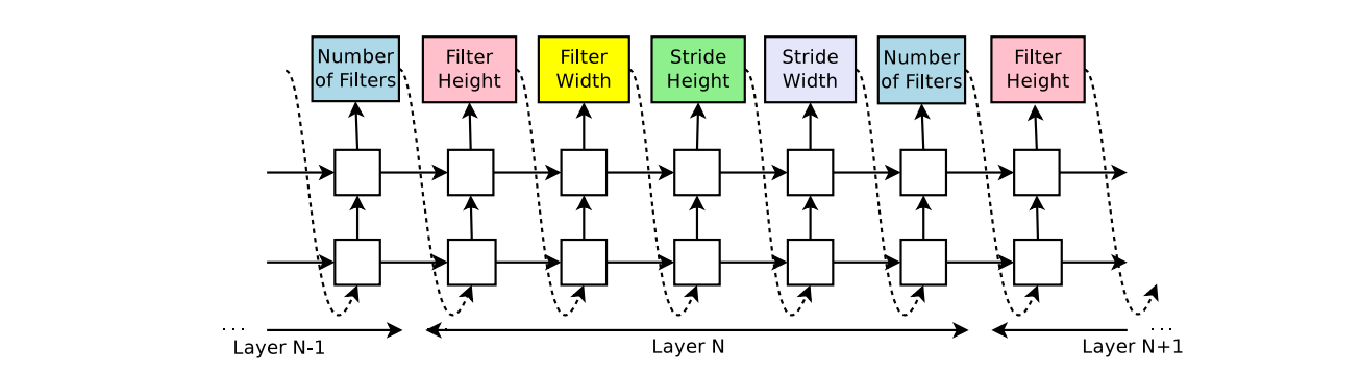
\includegraphics[width=0.95\textwidth]{figures/zoph-controller} \\
\href{https://openreview.net/forum?id=r1Ue8Hcxg}{\textcolor{blue}{Paper}}
\end{frame}

\begin{frame}{Making Neural Programming Architectures Generalize via Recursion}
\centering
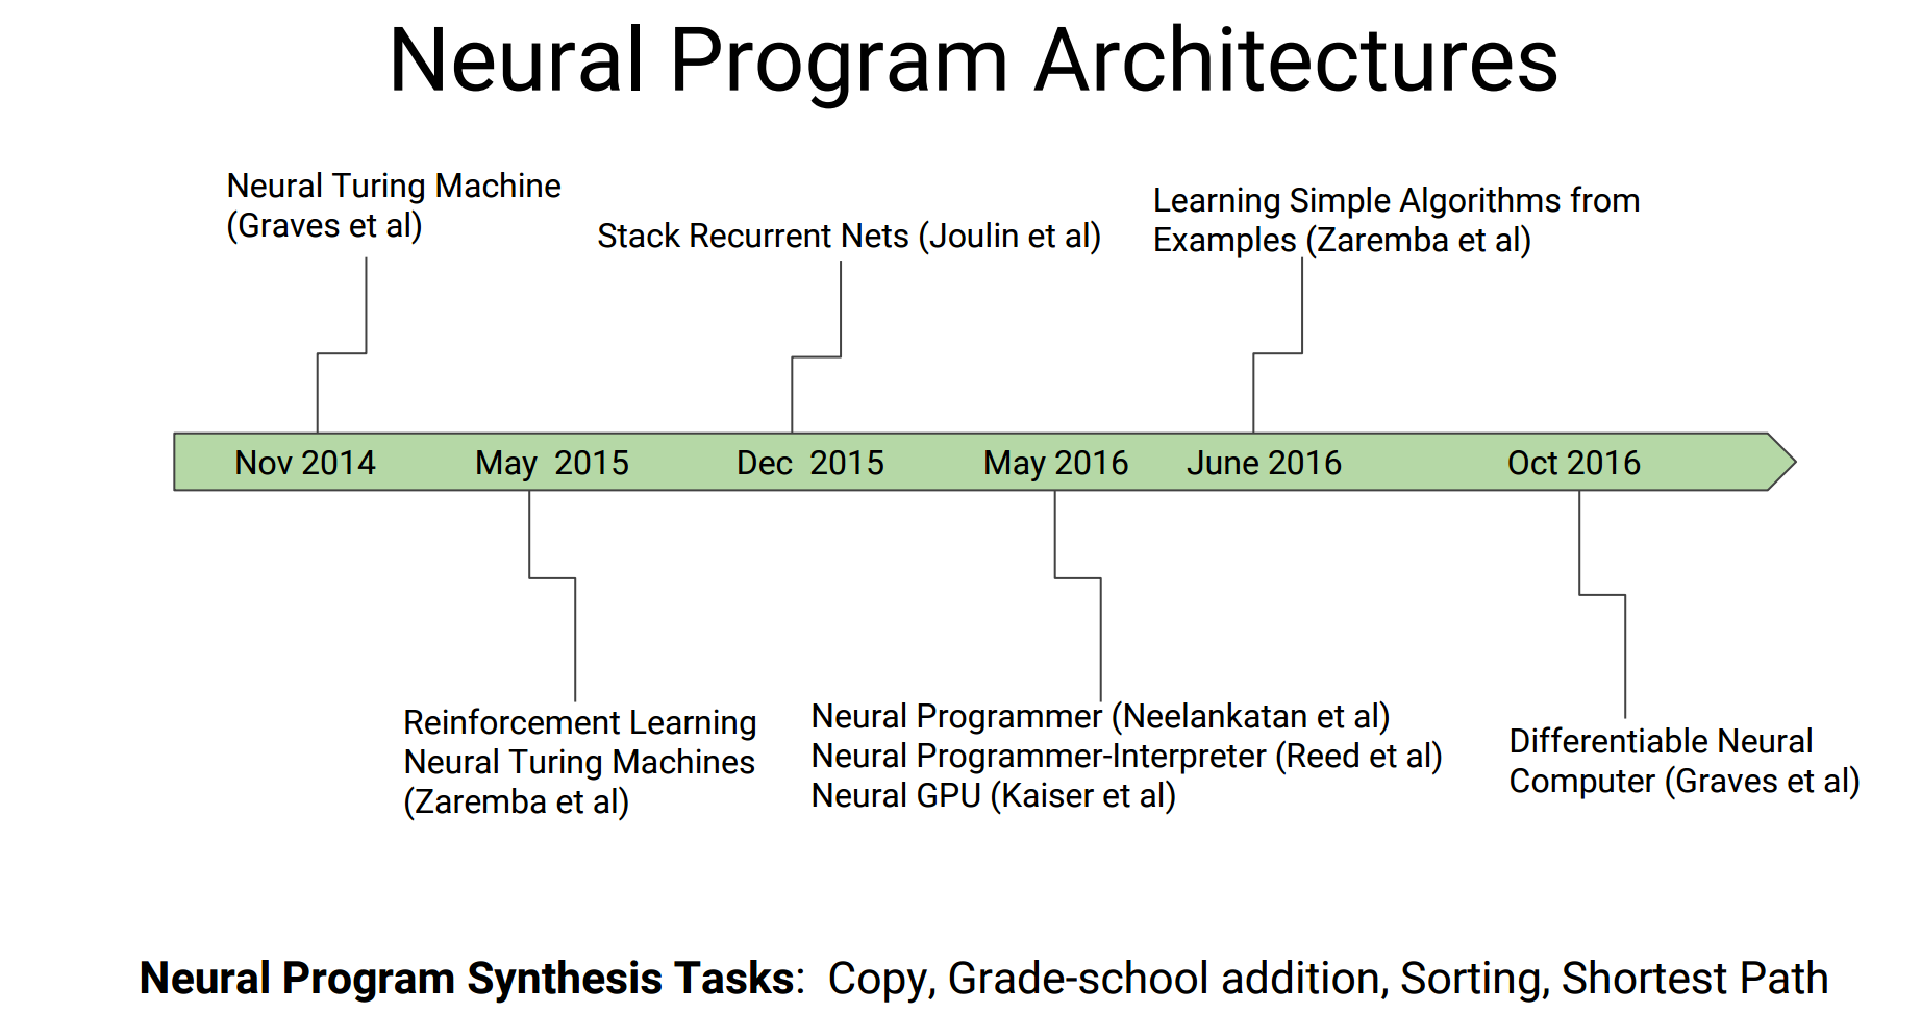
\includegraphics[width=0.9\textwidth]{figures/cai-np-architectures} \\
\href{https://openreview.net/forum?id=BkbY4psgg}{\textcolor{blue}{Paper}}
\end{frame}

\begin{frame}{Making Neural Programming Architectures Generalize via Recursion}
\centering
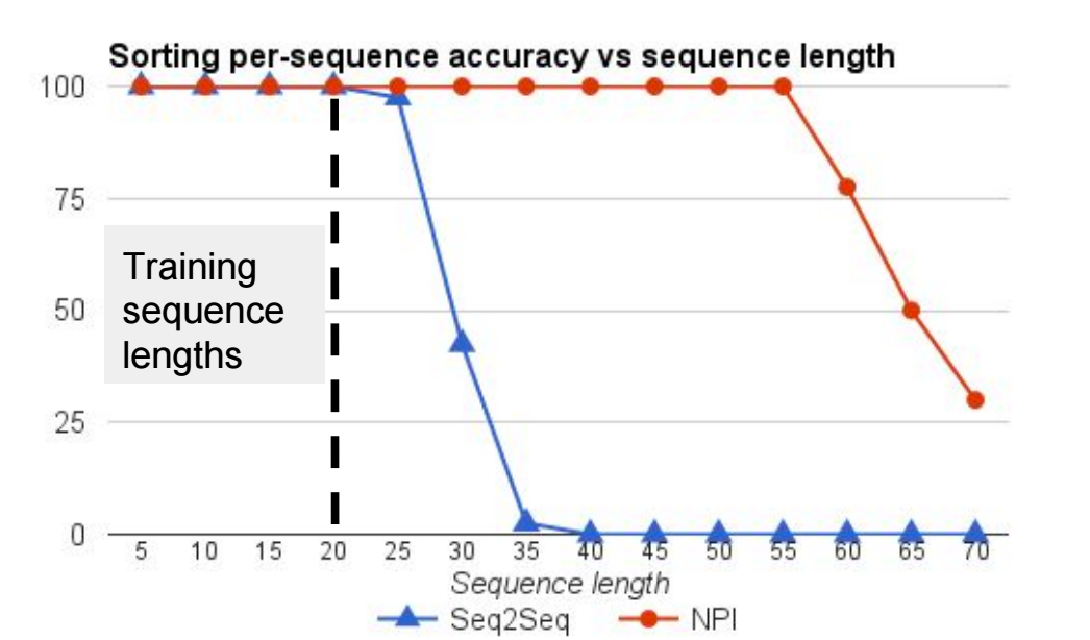
\includegraphics[width=0.9\textwidth]{figures/cai-npi-failure} \\
\href{https://openreview.net/forum?id=BkbY4psgg}{\textcolor{blue}{Paper}}
\end{frame}

\begin{frame}{Making Neural Programming Architectures Generalize via Recursion}
\centering
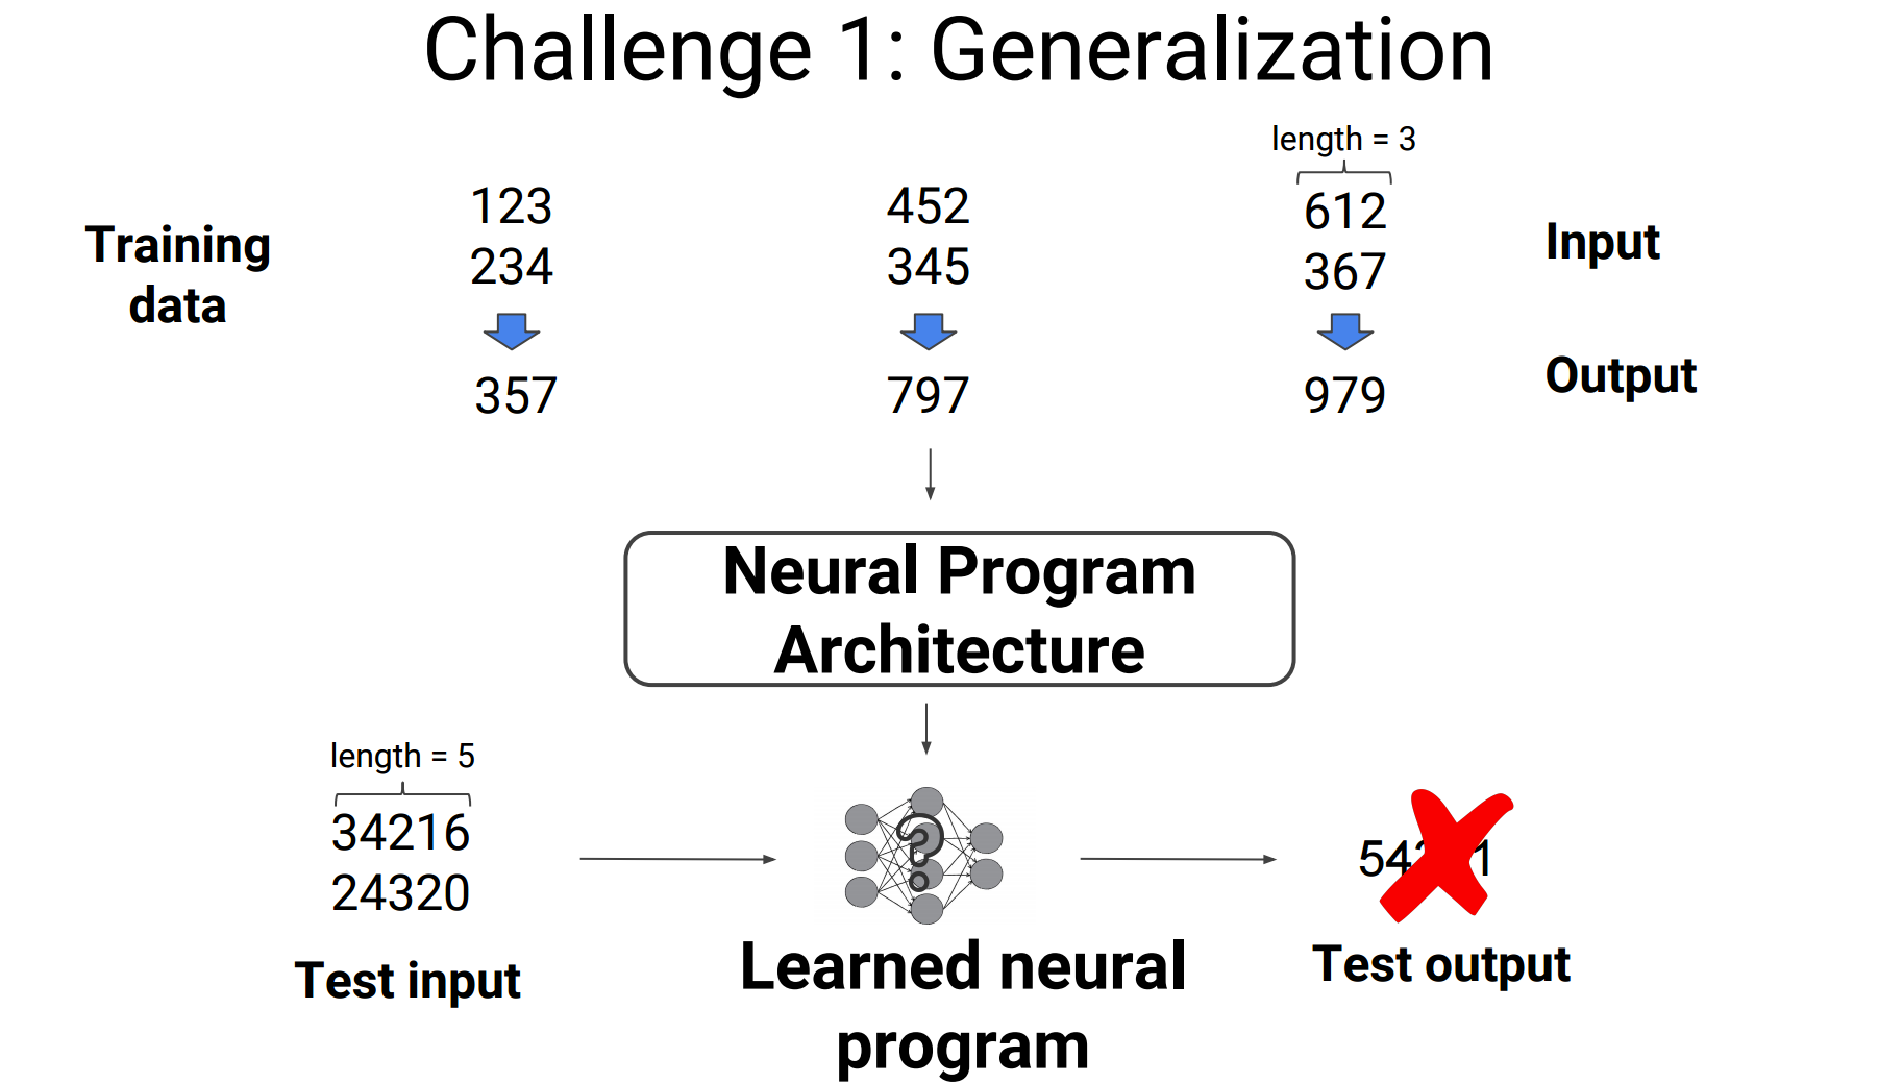
\includegraphics[width=0.9\textwidth]{figures/cai-challenge-generalization} \\
\href{https://openreview.net/forum?id=BkbY4psgg}{\textcolor{blue}{Paper}}
\end{frame}

\begin{frame}{Making Neural Programming Architectures Generalize via Recursion}
\centering
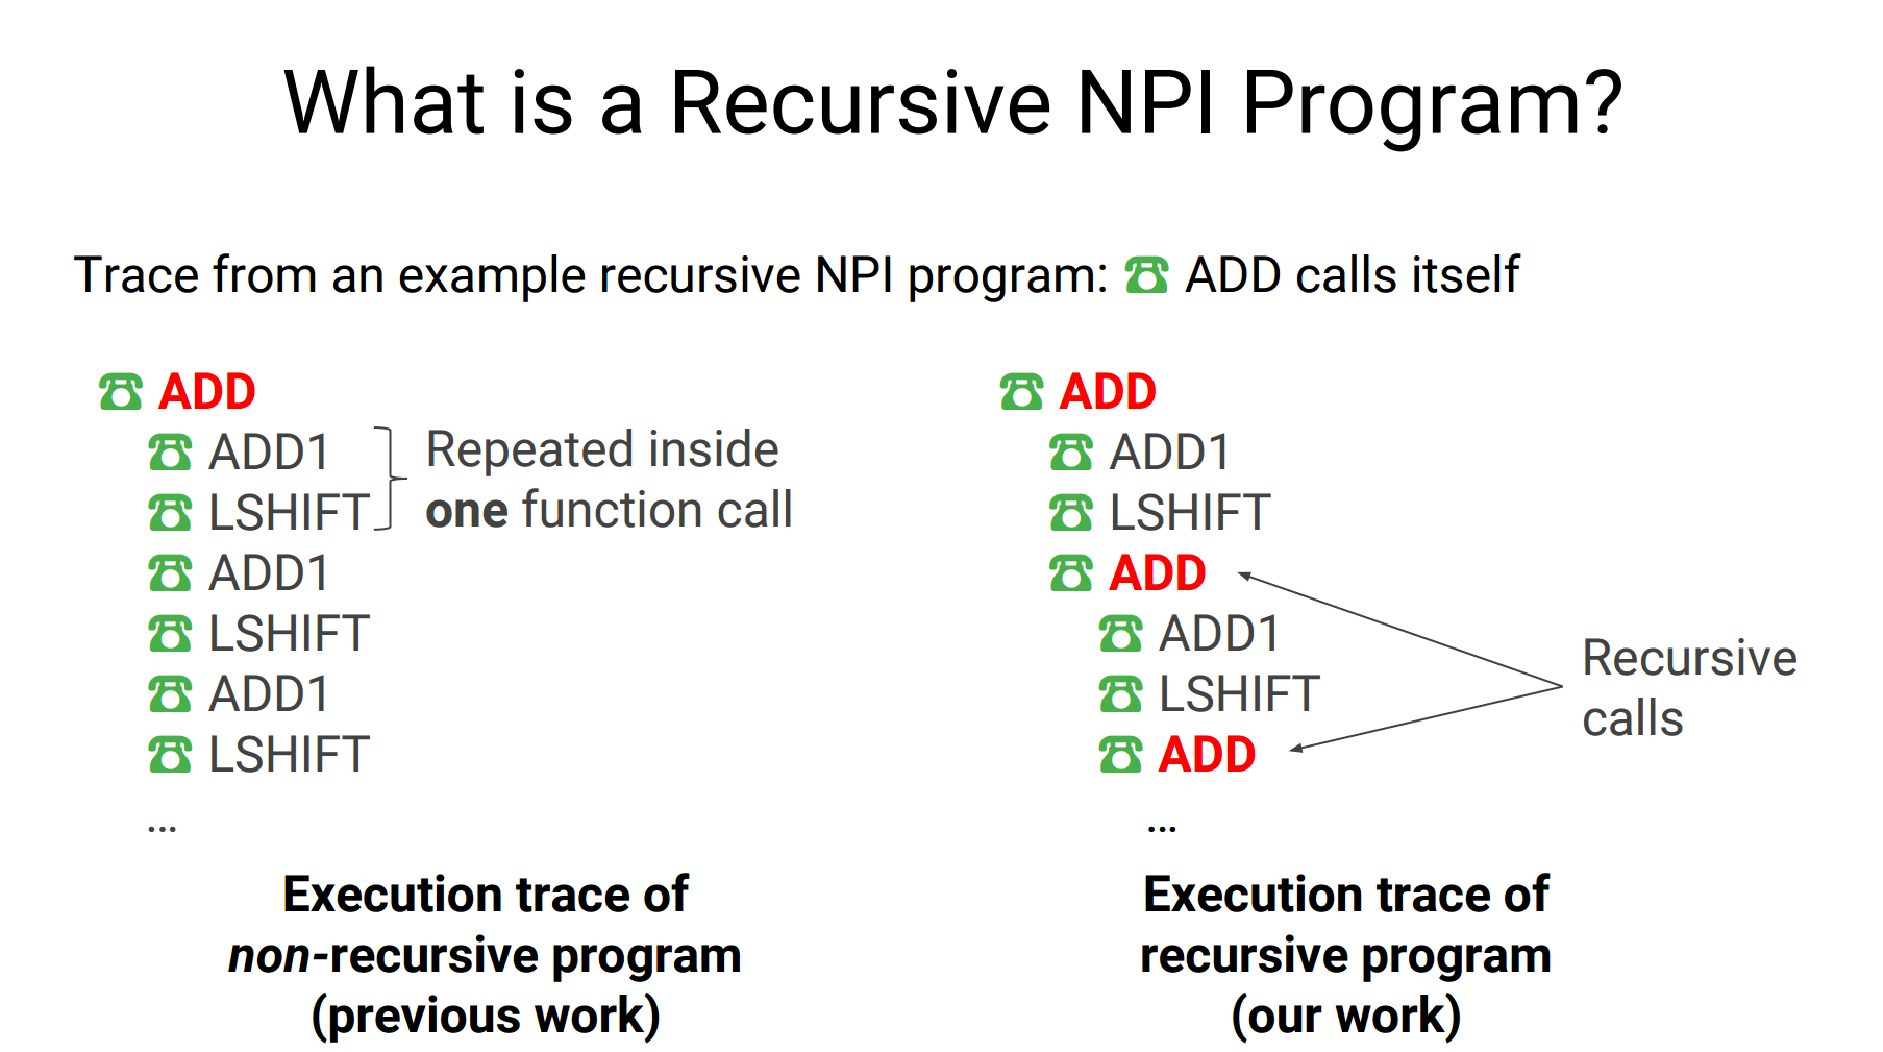
\includegraphics[width=0.9\textwidth]{figures/cai-recursive-npi} \\
\href{https://openreview.net/forum?id=BkbY4psgg}{\textcolor{blue}{Paper}}
\end{frame}

\begin{frame}{Making Neural Programming Architectures Generalize via Recursion}
\centering
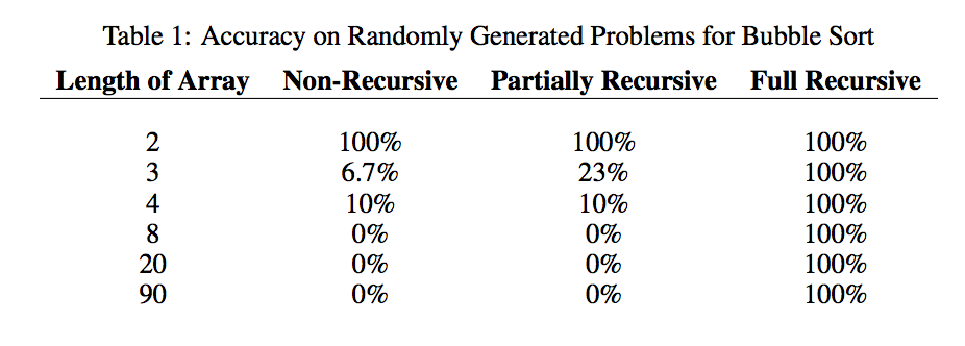
\includegraphics[width=0.9\textwidth]{figures/cai-results} \\
\href{https://openreview.net/forum?id=BkbY4psgg}{\textcolor{blue}{Paper}}
\end{frame}

\begin{frame}{Resources}
\begin{itemize}
\item Open Review for all submissions
  \begin{itemize}
  \item \href{https://openreview.net/group?id=ICLR.cc/2017/conference}{\textcolor{blue}{Conference track}}
  \item \href{https://openreview.net/group?id=ICLR.cc/2017/workshop}{\textcolor{blue}{Workshop track}}
  \end{itemize}
\item \href{https://www.facebook.com/pg/iclr.cc/videos/}{\textcolor{blue}{Videos of invited and contributed talks}}
\end{itemize}
\end{frame}

\end{document}
